\subsection{Variando el porcentaje de modificación del grafo causal}\label{exp1}

Se realiza una serie de experimentos donde se busca mostrar el comportamiento 
del método propuesto sobre subgrafos del grafo causal verdadero. Estos subgrafos son generados a partir del $\mathcal{D}$, alterándolo a diferentes niveles.

\subsubsection{Configuración experimental}

\begin{itemize}
    \item El espacio de estados es discreto, es decir, el agente puede
    obtener las variables $\mathcal{X}$ directamente del ambiente.
    \item Se prueba modificando el grafo $\mathcal{D}$ para obtener a los
    grafos $\mathcal{D'}$ y $\mathcal{D''}$ en tres niveles. El porcentaje de nivel de cambio se representa con el parámetro $p_{mod}$.
    Para cada nivel, el subgrafo $\mathcal{D'}$ se genera al remover un porcentaje $p_{mod}$ de las aristas en el grafo $\mathcal{D}$. Para producir $\mathcal{D''}$ se elimina $p_{mod}$ de las aristas y después, de la mitad de conexiones perdidas, se crean nuevas diferentes a las iniciales.
    \begin{itemize}
        \item Nivel bajo de modificación, $p_{mod} = 25 \%$.
        \item Nivel medio de modificación. $p_{mod} = 50 \%$.
        \item Nivel alto de modificación. $p_{mod} = 75 \%$
    \end{itemize}
    \item Se examina sobre los tres tipos de estructuras posibles: uno-a-uno, 
    causa común y efecto común. 
    \item Se prueba sobre ambientes deterministas y estocásticos.
    
    \item La tasa de exploración está dada por un $\delta = 0.5$ lo que indica que aproximadamente a mitad del entrenamiento la probabilidad de explotación alcanza su máximo valor.
\end{itemize}

\subsubsection{Objetivo}

Determinar si la información provista por un modelo
incompleto o parcialmente incorrecto ayuda y no
afecta negativamente el desempeño del algoritmo de RL.

\subsubsection{Hipótesis}

Dado que la información del modelo causal solo guía la selección
de acciones durante la exploración, entonces un grafo con escasos
datos correctos sigue siendo mejor que una búsqueda aleatoria \footnote{Hay que tener en cuenta que esto también es afectado por la tasa
de aprendizaje $\alpha$. Ésta se fija para todos los experimentos como $\alpha = 0.8$)}.
% En el
% peor caso, el algoritmo se comportaría como el método sin información adicional.


\subsubsection{Resultados}

Para comparar el desempeño de los distintos algoritmos propuestos
en las diferentes configuraciones del experimento
se evalúa la medida \textit{average} descrita anteriormente y se calcula una recompensa definida como óptima en cada configuración de los parámetros del experimento. Con esta información se puede establecer un umbral para saber qué método resuelve la tarea más rápido, a través de comparar el tamaño de la racha más larga ($>E=20$) en alcanzar y mantener la recompensa óptima.
De manera gráfica se puede ver el desempeño de los algoritmos
para los diferentes valores de $p_{mod}$ y tipo de ambiente en las Figuras \ref{fig:low-mod-det}, \ref{fig:low-mod-sto}, \ref{fig:med-mod-det}, \ref{fig:med-mod-sto},  \ref{fig:high-mod-det} y \ref{fig:high-mod-sto}. Además, en las tablas \ref{tab:one-to-one-pmod-det}, \ref{tab:one-to-one-pmod-sto}, \ref{tab:common-effect-pmod-det}, \ref{tab:common-effect-pmod-sto},
\ref{tab:common-cause-pmod-det} y \ref{tab:common-cause-pmod-sto}, se muestran los resultados de las pruebas estadísticas.


De acuerdo con las Figuras \ref{fig:low-mod-det}-\ref{fig:high-mod-sto} y las tablas
\ref{tab:one-to-one-pmod-det}-\ref{tab:common-cause-pmod-sto},
en la mayoría de los casos los algoritmos que utilizan conocimiento del grafo inician con una recompensa mayor y se estabilizan más rápido que el algoritmo Q-learning
sin información adicional en ambientes con transiciones deterministas y estocásticas.
En general, de acuerdo a los diagramas de la Figura \ref{fig:boxplots-pmod}, que muestran un resumen
de todos los resultados de las tablas, se puede notar que el 
usar el modelo completo supera a los demás métodos. Por otro lado, los
algoritmos $Q_3$ y $Q_4$ se comportan de manera similar.

Para el caso donde $p_{mod} = 25$, los algoritmos con información incompleta e incorrecta,
de las gráficas y tablas, se puede notar que comparten un rango de valores muy similar.
Esto puede ser debido 
a que la tasa de alteración del grafo es muy baja y  a que $N$ no toma
valores muy grandes, por lo que hay muy poca diferencia entre el grafo incompleto y el incorrecto. 
En el caso de $p_{mod} = 50$, se
puede notar que el desempeño de los algoritmos
con información incompleta e incorrecta se 
va moviendo en dirección a la curva del algoritmo
Q-learning sin información extra.
Finalmente, para $p_{mod} = 75$,  a pesar de haber modificado el grafo
causal en un porcentaje bastante alto, la poca información que queda y es correcta sigue siendo suficiente para alcanzar una recompensa mayor mucho más rápido, donde al menos es más notable para las estructuras de tipo causa común y de efecto común.
Existe un comportamiento extraño en las tareas con una estructura del tipo uno a uno. Se puede ver que entre más crece el valor de $N$ los algoritmos que utilizan el grafo tienden a decrecer en dirección al punto de transición en el que la explotación llega a su máximo valor. Sin embargo, una vez que pasa ese punto, los algoritmos se siguen comportando de manera superior al algoritmo clásico.

En los resultados de las estructuras uno a uno, en ambas configuraciones del ambiente y niveles de 
modificación en el grafo, el algoritmo con el grafo 
causal completo alcanza la recompensa esperada más rápido.
Para la mayoría de los casos de los otros dos algoritmos se 
resuelve la tarea antes que en el algoritmo $Q_1$. Las 
ocurrencias donde no se encontró una
diferencia con el algoritmo $Q_1$, en su mayoría son 
con respecto a modificaciones grandes (con $p_{mod}=75$) en el 
grafo causal.
En los problemas de efecto común, en el ambiente determinista y en todos niveles de  modificación en el grafo, el algoritmo con el grafo 
causal completo alcanza la recompensa esperada más rápido.
Este comportamiento no se repite en el estocástico,
en específico, sólo para un caso
Se repite el comportamiento donde
entre mayor sea $p_{mod}$, no se puede
encontrar una diferencia con $Q_1$.
Para el tipo de estructuras subyacentes de causa común en el problema, cambian 
un poco los resultados. En el caso del ambiente estocástico es donde 
en la mayoría de los casos los métodos propuestos
son mejores que el $Q_1$. Continua la misma tendencia
que al alterar bastante el grafo original para generar
el parcial y el que contiene relaciones ruidosas no se puede
concluir que exista diferencia con el Q-learning clásico.


\clearpage

% Please add the following required packages to your document preamble:
% \usepackage{multirow}
\begin{table}[]
\centering
\caption{Resumen de las pruebas estadísticas del t-test de Welch en las
estructuras uno a uno en un ambiente determinista. Se muestra la media y desviación estándar $std$ del número 
de episodios que tarda en alcanzar la recompensa óptima, para los cuatro métodos, los diferentes número de luces $N$, y modificaciones del grafo $p_{mod}$ (para las estructuras que son usadas en $Q_2$ y $Q_3$). Además, se pone la información
de la prueba estadística, el estadístico $t$, los grados de libertad $df$, el nivel
de significacia $p$, la hipótesis nula $h_0$ (que corresponde a si noy hay diferencia entre $Q_1$ y el método correspondiente) y el tamaño de efecto $d$ de \citet{cohen2013statistical}.}
\label{tab:one-to-one-pmod-det}
\begin{tabular}{|l|l|l|l|l|l|l|l|l|l|}
\hline
$N$ & $p_{mod}$ & Alg & Media & $std$ & $t$ & $df$ & $p$ & $h_0$ & $d$ \\ \hline
\multirow{12}{*}{5} & \multirow{4}{*}{25} & $Q_1$ & 10000.00 & 0.00 & \multicolumn{5}{l|}{} \\ \cline{3-10} 
 &  & $Q_2$ & 4992.00 & 2249.06 & -6.68 & 9.00 & 0.00 & rechazada & 2.99 \\ \cline{3-10} 
 &  & $Q_3$ & 8062.00 & 1360.22 & -4.27 & 9.00 & 0.00 & rechazada & 1.91 \\ \cline{3-10} 
 &  & $Q_4$ & 8590.00 & 1062.31 & -3.98 & 9.00 & 0.00 & rechazada & 1.78 \\ \cline{2-10} 
 & \multirow{4}{*}{50} & $Q_1$ & 10000.00 & 0.00 & \multicolumn{5}{l|}{} \\ \cline{3-10} 
 &  & $Q_2$ & 5178.00 & 1621.47 & -8.92 & 9.00 & 0.00 & rechazada & 3.99 \\ \cline{3-10} 
 &  & $Q_3$ & 9396.00 & 1044.02 & -1.74 & 9.00 & 0.12 & aceptada & 0.78 \\ \cline{3-10} 
 &  & $Q_4$ & 9510.00 & 827.78 & -1.78 & 9.00 & 0.11 & aceptada & 0.79 \\ \cline{2-10} 
 & \multirow{4}{*}{75} & $Q_1$ & 10000.00 & 0.00 & \multicolumn{5}{l|}{} \\ \cline{3-10} 
 &  & $Q_2$ & 5326.00 & 1737.29 & -8.07 & 9.00 & 0.00 & rechazada & 3.61 \\ \cline{3-10} 
 &  & $Q_3$ & 9848.00 & 312.31 & -1.46 & 9.00 & 0.18 & aceptada & 0.65 \\ \cline{3-10} 
 &  & $Q_4$ & 10000.00 & 0.00 & 0.0 & 18.0 & 1.0 & aceptada & 0.0 \\ \hline
\multirow{12}{*}{7} & \multirow{4}{*}{25} & $Q_1$ & 10000.00 & 0.00 & \multicolumn{5}{l|}{} \\ \cline{3-10} 
 &  & $Q_2$ & 6364.00 & 1381.50 & -7.90 & 9.00 & 0.00 & rechazada & 3.53 \\ \cline{3-10} 
 &  & $Q_3$ & 7794.00 & 1016.23 & -6.51 & 9.00 & 0.00 & rechazada & 2.91 \\ \cline{3-10} 
 &  & $Q_4$ & 7724.00 & 1142.87 & -5.97 & 9.00 & 0.00 & rechazada & 2.67 \\ \cline{2-10} 
 & \multirow{4}{*}{50} & $Q_1$ & 10000.00 & 0.00 & \multicolumn{5}{l|}{} \\ \cline{3-10} 
 &  & $Q_2$ & 7676.00 & 957.91 & -7.28 & 9.00 & 0.00 & rechazada & 3.25 \\ \cline{3-10} 
 &  & $Q_3$ & 8206.00 & 1116.39 & -4.82 & 9.00 & 0.00 & rechazada & 2.16 \\ \cline{3-10} 
 &  & $Q_4$ & 8182.00 & 1238.37 & -4.40 & 9.00 & 0.00 & rechazada & 1.97 \\ \cline{2-10} 
 & \multirow{4}{*}{75} & $Q_1$ & 10000.00 & 0.00 & \multicolumn{5}{l|}{} \\ \cline{3-10} 
 &  & $Q_2$ & 6998.00 & 1228.31 & -7.33 & 9.00 & 0.00 & rechazada & 3.28 \\ \cline{3-10} 
 &  & $Q_3$ & 9074.00 & 1253.16 & -2.22 & 9.00 & 0.05 & aceptada & 0.99 \\ \cline{3-10} 
 &  & $Q_4$ & 9822.00 & 534.00 & -1.00 & 9.00 & 0.34 & aceptada & 0.45 \\ \hline
\multirow{12}{*}{9} & \multirow{4}{*}{25} & $Q_1$ & 20000.00 & 0.00 & \multicolumn{5}{l|}{} \\ \cline{3-10} 
 &  & $Q_2$ & 16584.00 & 747.25 & -13.71 & 9.00 & 0.00 & rechazada & 6.13 \\ \cline{3-10} 
 &  & $Q_3$ & 16984.00 & 1495.99 & -6.05 & 9.00 & 0.00 & rechazada & 2.70 \\ \cline{3-10} 
 &  & $Q_4$ & 17350.00 & 1686.59 & -4.71 & 9.00 & 0.00 & rechazada & 2.11 \\ \cline{2-10} 
 & \multirow{4}{*}{50} & $Q_1$ & 20000.00 & 0.00 & \multicolumn{5}{l|}{} \\ \cline{3-10} 
 &  & $Q_2$ & 17330.00 & 1462.33 & -5.48 & 9.00 & 0.00 & rechazada & 2.45 \\ \cline{3-10} 
 &  & $Q_3$ & 17992.00 & 1458.39 & -4.13 & 9.00 & 0.00 & rechazada & 1.85 \\ \cline{3-10} 
 &  & $Q_4$ & 18908.00 & 1105.67 & -2.96 & 9.00 & 0.02 & rechazada & 1.33 \\ \cline{2-10} 
 & \multirow{4}{*}{75} & $Q_1$ & 20000.00 & 0.00 & \multicolumn{5}{l|}{} \\ \cline{3-10} 
 &  & $Q_2$ & 17254.00 & 1352.57 & -6.09 & 9.00 & 0.00 & rechazada & 2.72 \\ \cline{3-10} 
 &  & $Q_3$ & 18408.00 & 1587.00 & -3.01 & 9.00 & 0.01 & rechazada & 1.35 \\ \cline{3-10} 
 &  & $Q_4$ & 20000.00 & 0.00 & 0.0 & 18.0 & 1.0 & aceptada & 0.0 \\ \hline
\end{tabular}
\end{table}


\clearpage

% Please add the following required packages to your document preamble:
% \usepackage{multirow}
\begin{table}[]
\centering
\caption{Resumen de las pruebas estadísticas del t-test de Welch en las
estructuras uno a uno en un ambiente estocástico. Se muestra la media y desviación estándar $std$ del número 
de episodios que tarda en alcanzar la recompensa óptima, para los cuatro métodos, los diferentes número de luces $N$, y modificaciones del grafo $p_{mod}$ (para las estructuras que son usadas en $Q_2$ y $Q_3$). Además, se pone la información
de la prueba estadística, el estadístico $t$, los grados de libertad $df$, el nivel
de significacia $p$, la hipótesis nula $h_0$ (que corresponde a si noy hay diferencia entre $Q_1$ y el método correspondiente) y el tamaño de efecto $d$ de \citet{cohen2013statistical}.}
\label{tab:one-to-one-pmod-sto}
\begin{tabular}{|l|l|l|l|l|l|l|l|l|l|}
\hline
$N$ & $p_{mod}$ & Alg & Media & $std$ & $t$ & $df$ & $p$ & $h_0$ & $d$ \\ \hline
\multirow{12}{*}{5} & \multirow{4}{*}{25} & $Q_1$ & 10000.00 & 0.00 & \multicolumn{5}{l|}{} \\ \cline{3-10} 
 &  & $Q_2$ & 6156.00 & 2333.83 & -4.94 & 9.00 & 0.00 & rechazada & 2.21 \\ \cline{3-10} 
 &  & $Q_3$ & 6176.00 & 2330.42 & -4.92 & 9.00 & 0.00 & rechazada & 2.20 \\ \cline{3-10} 
 &  & $Q_4$ & 8000.00 & 951.97 & -6.30 & 9.00 & 0.00 & rechazada & 2.82 \\ \cline{2-10} 
 & \multirow{4}{*}{50} & $Q_1$ & 10000.00 & 0.00 & \multicolumn{5}{l|}{} \\ \cline{3-10} 
 &  & $Q_2$ & 5162.00 & 2521.42 & -5.76 & 9.00 & 0.00 & rechazada & 2.57 \\ \cline{3-10} 
 &  & $Q_3$ & 7646.00 & 1047.86 & -6.74 & 9.00 & 0.00 & rechazada & 3.01 \\ \cline{3-10} 
 &  & $Q_4$ & 8062.00 & 979.73 & -5.93 & 9.00 & 0.00 & rechazada & 2.65 \\ \cline{2-10} 
 & \multirow{4}{*}{75} & $Q_1$ & 10000.00 & 0.00 & \multicolumn{5}{l|}{} \\ \cline{3-10} 
 &  & $Q_2$ & 4368.00 & 2900.43 & -5.83 & 9.00 & 0.00 & rechazada & 2.61 \\ \cline{3-10} 
 &  & $Q_3$ & 8298.00 & 1307.10 & -3.91 & 9.00 & 0.00 & rechazada & 1.75 \\ \cline{3-10} 
 &  & $Q_4$ & 9036.00 & 1503.03 & -1.92 & 9.00 & 0.09 & aceptada & 0.86 \\ \hline
\multirow{12}{*}{7} & \multirow{4}{*}{25} & $Q_1$ & 10000.00 & 0.00 & \multicolumn{5}{l|}{} \\ \cline{3-10} 
 &  & $Q_2$ & 4028.00 & 1805.66 & -9.92 & 9.00 & 0.00 & rechazada & 4.44 \\ \cline{3-10} 
 &  & $Q_3$ & 7602.00 & 1222.54 & -5.88 & 9.00 & 0.00 & rechazada & 2.63 \\ \cline{3-10} 
 &  & $Q_4$ & 7854.00 & 448.83 & -14.34 & 9.00 & 0.00 & rechazada & 6.41 \\ \cline{2-10} 
 & \multirow{4}{*}{50} & $Q_1$ & 9946.00 & 162.00 & \multicolumn{5}{l|}{} \\ \cline{3-10} 
 &  & $Q_2$ & 4766.00 & 1854.83 & -8.35 & 9.14 & 0.00 & rechazada & 3.73 \\ \cline{3-10} 
 &  & $Q_3$ & 8214.00 & 666.16 & -7.58 & 10.06 & 0.00 & rechazada & 3.39 \\ \cline{3-10} 
 &  & $Q_4$ & 7776.00 & 1054.51 & -6.10 & 9.42 & 0.00 & rechazada & 2.73 \\ \cline{2-10} 
 & \multirow{4}{*}{75} & $Q_1$ & 10000.00 & 0.00 & \multicolumn{5}{l|}{} \\ \cline{3-10} 
 &  & $Q_2$ & 5040.00 & 2513.04 & -5.92 & 9.00 & 0.00 & rechazada & 2.65 \\ \cline{3-10} 
 &  & $Q_3$ & 9850.00 & 450.00 & -1.00 & 9.00 & 0.34 & aceptada & 0.45 \\ \cline{3-10} 
 &  & $Q_4$ & 9720.00 & 840.00 & -1.00 & 9.00 & 0.34 & aceptada & 0.45 \\ \hline
\multirow{12}{*}{9} & \multirow{4}{*}{25} & $Q_1$ & 20000.00 & 0.00 & \multicolumn{5}{l|}{} \\ \cline{3-10} 
 &  & $Q_2$ & 15480.00 & 1256.76 & -10.79 & 9.00 & 0.00 & rechazada & 4.83 \\ \cline{3-10} 
 &  & $Q_3$ & 16334.00 & 823.94 & -13.35 & 9.00 & 0.00 & rechazada & 5.97 \\ \cline{3-10} 
 &  & $Q_4$ & 17052.00 & 1414.05 & -6.25 & 9.00 & 0.00 & rechazada & 2.80 \\ \cline{2-10} 
 & \multirow{4}{*}{50} & $Q_1$ & 20000.00 & 0.00 & \multicolumn{5}{l|}{} \\ \cline{3-10} 
 &  & $Q_2$ & 15928.00 & 996.08 & -12.26 & 9.00 & 0.00 & rechazada & 5.48 \\ \cline{3-10} 
 &  & $Q_3$ & 17132.00 & 1732.42 & -4.97 & 9.00 & 0.00 & rechazada & 2.22 \\ \cline{3-10} 
 &  & $Q_4$ & 17646.00 & 2257.20 & -3.13 & 9.00 & 0.01 & rechazada & 1.40 \\ \cline{2-10} 
 & \multirow{4}{*}{75} & $Q_1$ & 20000.00 & 0.00 & \multicolumn{5}{l|}{} \\ \cline{3-10} 
 &  & $Q_2$ & 15610.00 & 792.53 & -16.62 & 9.00 & 0.00 & rechazada & 7.43 \\ \cline{3-10} 
 &  & $Q_3$ & 18128.00 & 1328.49 & -4.23 & 9.00 & 0.00 & rechazada & 1.89 \\ \cline{3-10} 
 &  & $Q_4$ & 17958.00 & 2487.25 & -2.46 & 9.00 & 0.04 & rechazada & 1.10 \\ \hline
\end{tabular}
\end{table}

\clearpage

% Please add the following required packages to your document preamble:
% \usepackage{multirow}
\begin{table}[]
\centering
\caption{Resumen de las pruebas estadísticas del t-test de Welch en las
estructuras de efecto común en un ambiente determinista. Se muestra la media y desviación estándar $std$ del número 
de episodios que tarda en alcanzar la recompensa óptima, para los cuatro métodos, los diferentes número de luces $N$, y modificaciones del grafo $p_{mod}$ (para las estructuras que son usadas en $Q_2$ y $Q_3$). Además, se pone la información
de la prueba estadística, el estadístico $t$, los grados de libertad $df$, el nivel
de significacia $p$, la hipótesis nula $h_0$ (que corresponde a si noy hay diferencia entre $Q_1$ y el método correspondiente) y el tamaño de efecto $d$ de \citet{cohen2013statistical}.}
\label{tab:common-effect-pmod-det}
\begin{tabular}{|l|l|l|l|l|l|l|l|l|l|}
\hline
$N$ & $p_{mod}$ & Alg & Media & $std$ & $t$ & $df$ & $p$ & $h_0$ & $d$ \\ \hline
\multirow{12}{*}{5} & \multirow{4}{*}{25} & $Q_1$ & 9640.00 & 586.24 & \multicolumn{5}{l|}{} \\ \cline{3-10} 
 &  & $Q_2$ & 5908.00 & 4199.51 & -2.64 & 9.35 & 0.03 & rechazada & 1.18 \\ \cline{3-10} 
 &  & $Q_3$ & 6574.00 & 3699.45 & -2.46 & 9.45 & 0.04 & rechazada & 1.10 \\ \cline{3-10} 
 &  & $Q_4$ & 7718.00 & 3401.68 & -1.67 & 9.53 & 0.13 & aceptada & 0.75 \\ \cline{2-10} 
 & \multirow{4}{*}{50} & $Q_1$ & 9760.00 & 493.88 & \multicolumn{5}{l|}{} \\ \cline{3-10} 
 &  & $Q_2$ & 6638.00 & 3129.82 & -2.96 & 9.45 & 0.02 & rechazada & 1.32 \\ \cline{3-10} 
 &  & $Q_3$ & 8682.00 & 2103.53 & -1.50 & 9.99 & 0.17 & aceptada & 0.67 \\ \cline{3-10} 
 &  & $Q_4$ & 9650.00 & 550.65 & -0.45 & 17.79 & 0.66 & aceptada & 0.20 \\ \cline{2-10} 
 & \multirow{4}{*}{75} & $Q_1$ & 9952.00 & 144.00 & \multicolumn{5}{l|}{} \\ \cline{3-10} 
 &  & $Q_2$ & 5346.00 & 2790.90 & -4.94 & 9.05 & 0.00 & rechazada & 2.21 \\ \cline{3-10} 
 &  & $Q_3$ & 9100.00 & 2700.00 & -0.95 & 9.05 & 0.37 & aceptada & 0.42 \\ \cline{3-10} 
 &  & $Q_4$ & 9100.00 & 2700.00 & -0.95 & 9.05 & 0.37 & aceptada & 0.42 \\ \hline
\multirow{12}{*}{7} & \multirow{4}{*}{25} & $Q_1$ & 9882.00 & 238.07 & \multicolumn{5}{l|}{} \\ \cline{3-10} 
 &  & $Q_2$ & 5088.00 & 4093.05 & -3.51 & 9.06 & 0.01 & rechazada & 1.57 \\ \cline{3-10} 
 &  & $Q_3$ & 5936.00 & 4180.45 & -2.83 & 9.06 & 0.02 & rechazada & 1.26 \\ \cline{3-10} 
 &  & $Q_4$ & 6110.00 & 4007.58 & -2.82 & 9.06 & 0.02 & rechazada & 1.26 \\ \cline{2-10} 
 & \multirow{4}{*}{50} & $Q_1$ & 9888.00 & 336.00 & \multicolumn{5}{l|}{} \\ \cline{3-10} 
 &  & $Q_2$ & 5350.00 & 3915.97 & -3.46 & 9.13 & 0.01 & rechazada & 1.55 \\ \cline{3-10} 
 &  & $Q_3$ & 9146.00 & 1719.00 & -1.27 & 9.69 & 0.23 & aceptada & 0.57 \\ \cline{3-10} 
 &  & $Q_4$ & 9024.00 & 2684.25 & -0.96 & 9.28 & 0.36 & aceptada & 0.43 \\ \cline{2-10} 
 & \multirow{4}{*}{75} & $Q_1$ & 9640.00 & 557.71 & \multicolumn{5}{l|}{} \\ \cline{3-10} 
 &  & $Q_2$ & 4846.00 & 3776.21 & -3.77 & 9.39 & 0.00 & rechazada & 1.68 \\ \cline{3-10} 
 &  & $Q_3$ & 9492.00 & 664.96 & -0.51 & 17.47 & 0.62 & aceptada & 0.23 \\ \cline{3-10} 
 &  & $Q_4$ & 9296.00 & 999.19 & -0.90 & 14.11 & 0.38 & aceptada & 0.40 \\ \hline
\multirow{12}{*}{9} & \multirow{4}{*}{25} & $Q_1$ & 19472.00 & 859.73 & \multicolumn{5}{l|}{} \\ \cline{3-10} 
 &  & $Q_2$ & 11604.00 & 7828.16 & -3.00 & 9.22 & 0.01 & rechazada & 1.34 \\ \cline{3-10} 
 &  & $Q_3$ & 12200.00 & 7886.63 & -2.75 & 9.21 & 0.02 & rechazada & 1.23 \\ \cline{3-10} 
 &  & $Q_4$ & 15102.00 & 5861.00 & -2.21 & 9.39 & 0.05 & aceptada & 0.99 \\ \cline{2-10} 
 & \multirow{4}{*}{50} & $Q_1$ & 19452.00 & 731.97 & \multicolumn{5}{l|}{} \\ \cline{3-10} 
 &  & $Q_2$ & 11286.00 & 6356.81 & -3.83 & 9.24 & 0.00 & rechazada & 1.71 \\ \cline{3-10} 
 &  & $Q_3$ & 18616.00 & 1878.87 & -1.24 & 11.67 & 0.24 & aceptada & 0.56 \\ \cline{3-10} 
 &  & $Q_4$ & 19246.00 & 1364.58 & -0.40 & 13.78 & 0.70 & aceptada & 0.18 \\ \cline{2-10} 
 & \multirow{4}{*}{75} & $Q_1$ & 19416.00 & 785.05 & \multicolumn{5}{l|}{} \\ \cline{3-10} 
 &  & $Q_2$ & 10980.00 & 7079.43 & -3.55 & 9.22 & 0.01 & rechazada & 1.59 \\ \cline{3-10} 
 &  & $Q_3$ & 19084.00 & 1180.33 & -0.70 & 15.66 & 0.49 & aceptada & 0.31 \\ \cline{3-10} 
 &  & $Q_4$ & 19364.00 & 789.37 & -0.14 & 18.00 & 0.89 & aceptada & 0.06 \\ \hline
\end{tabular}
\end{table}

\clearpage
% Please add the following required packages to your document preamble:
% \usepackage{multirow}
\begin{table}[]
\centering
\caption{Resumen de las pruebas estadísticas del t-test de Welch en las
estructuras de efecto común en un ambiente estocástico. Se muestra la media y desviación estándar $std$ del número 
de episodios que tarda en alcanzar la recompensa óptima, para los cuatro métodos, los diferentes número de luces $N$, y modificaciones del grafo $p_{mod}$ (para las estructuras que son usadas en $Q_2$ y $Q_3$). Además, se pone la información
de la prueba estadística, el estadístico $t$, los grados de libertad $df$, el nivel
de significacia $p$, la hipótesis nula $h_0$ (que corresponde a si noy hay diferencia entre $Q_1$ y el método correspondiente) y el tamaño de efecto $d$ de \citet{cohen2013statistical}.}
\label{tab:common-effect-pmod-sto}
\begin{tabular}{|l|l|l|l|l|l|l|l|l|l|}
\hline
$N$ & $p_{mod}$ & Alg & Media & std & $t$ & $df$ & $p$ & $h_0$ & $d$ \\ \hline
\multirow{12}{*}{5} & \multirow{4}{*}{25} & $Q_1$ & 8676.00 & 1694.93 & \multicolumn{5}{l|}{} \\ \cline{3-10} 
 &  & $Q_2$ & 6038.00 & 3701.40 & -1.94 & 12.62 & 0.07 & aceptada & 0.87 \\ \cline{3-10} 
 &  & $Q_3$ & 5940.00 & 3875.80 & -1.94 & 12.32 & 0.08 & aceptada & 0.87 \\ \cline{3-10} 
 &  & $Q_4$ & 5780.00 & 3818.38 & -2.08 & 12.41 & 0.06 & aceptada & 0.93 \\ \cline{2-10} 
 & \multirow{4}{*}{50} & $Q_1$ & 9832.00 & 504.00 & \multicolumn{5}{l|}{} \\ \cline{3-10} 
 &  & $Q_2$ & 4918.00 & 2569.22 & -5.63 & 9.69 & 0.00 & rechazada & 2.52 \\ \cline{3-10} 
 &  & $Q_3$ & 6922.00 & 2752.26 & -3.12 & 9.60 & 0.01 & rechazada & 1.40 \\ \cline{3-10} 
 &  & $Q_4$ & 8950.00 & 1318.55 & -1.87 & 11.57 & 0.09 & aceptada & 0.84 \\ \cline{2-10} 
 & \multirow{4}{*}{75} & $Q_1$ & 9540.00 & 787.71 & \multicolumn{5}{l|}{} \\ \cline{3-10} 
 &  & $Q_2$ & 5122.00 & 3747.85 & -3.46 & 9.79 & 0.01 & rechazada & 1.55 \\ \cline{3-10} 
 &  & $Q_3$ & 8384.00 & 2572.06 & -1.29 & 10.67 & 0.22 & aceptada & 0.58 \\ \cline{3-10} 
 &  & $Q_4$ & 7938.00 & 3554.52 & -1.32 & 9.88 & 0.22 & aceptada & 0.59 \\ \hline
\multirow{12}{*}{7} & \multirow{4}{*}{25} & $Q_1$ & 9254.00 & 999.88 & \multicolumn{5}{l|}{} \\ \cline{3-10} 
 &  & $Q_2$ & 4110.00 & 3178.22 & -4.63 & 10.76 & 0.00 & rechazada & 2.07 \\ \cline{3-10} 
 &  & $Q_3$ & 6616.00 & 3190.51 & -2.37 & 10.75 & 0.04 & rechazada & 1.06 \\ \cline{3-10} 
 &  & $Q_4$ & 4022.00 & 3093.21 & -4.83 & 10.86 & 0.00 & rechazada & 2.16 \\ \cline{2-10} 
 & \multirow{4}{*}{50} & $Q_1$ & 9332.00 & 1137.20 & \multicolumn{5}{l|}{} \\ \cline{3-10} 
 &  & $Q_2$ & 3042.00 & 2402.96 & -7.10 & 12.84 & 0.00 & rechazada & 3.17 \\ \cline{3-10} 
 &  & $Q_3$ & 6790.00 & 3211.87 & -2.24 & 11.22 & 0.05 & rechazada & 1.00 \\ \cline{3-10} 
 &  & $Q_4$ & 7886.00 & 2595.52 & -1.53 & 12.33 & 0.15 & aceptada & 0.68 \\ \cline{2-10} 
 & \multirow{4}{*}{75} & $Q_1$ & 8866.00 & 1197.47 & \multicolumn{5}{l|}{} \\ \cline{3-10} 
 &  & $Q_2$ & 3938.00 & 3751.51 & -3.75 & 10.82 & 0.00 & rechazada & 1.68 \\ \cline{3-10} 
 &  & $Q_3$ & 8832.00 & 1117.75 & -0.06 & 17.92 & 0.95 & aceptada & 0.03 \\ \cline{3-10} 
 &  & $Q_4$ & 8476.00 & 1378.54 & -0.64 & 17.65 & 0.53 & aceptada & 0.29 \\ \hline
\multirow{12}{*}{9} & \multirow{4}{*}{25} & $Q_1$ & 17484.00 & 2808.57 & \multicolumn{5}{l|}{} \\ \cline{3-10} 
 &  & $Q_2$ & 5866.00 & 5459.41 & -5.68 & 13.45 & 0.00 & rechazada & 2.54 \\ \cline{3-10} 
 &  & $Q_3$ & 15000.00 & 3595.27 & -1.63 & 17.00 & 0.12 & aceptada & 0.73 \\ \cline{3-10} 
 &  & $Q_4$ & 11748.00 & 6873.61 & -2.32 & 11.92 & 0.04 & rechazada & 1.04 \\ \cline{2-10} 
 & \multirow{4}{*}{50} & $Q_1$ & 19098.00 & 1393.77 & \multicolumn{5}{l|}{} \\ \cline{3-10} 
 &  & $Q_2$ & 6740.00 & 5322.11 & -6.74 & 10.23 & 0.00 & rechazada & 3.01 \\ \cline{3-10} 
 &  & $Q_3$ & 15122.00 & 2166.66 & -4.63 & 15.36 & 0.00 & rechazada & 2.07 \\ \cline{3-10} 
 &  & $Q_4$ & 16230.00 & 2243.41 & -3.26 & 15.05 & 0.01 & rechazada & 1.46 \\ \cline{2-10} 
 & \multirow{4}{*}{75} & $Q_1$ & 17718.00 & 2934.67 & \multicolumn{5}{l|}{} \\ \cline{3-10} 
 &  & $Q_2$ & 6030.00 & 5621.74 & -5.53 & 13.57 & 0.00 & rechazada & 2.47 \\ \cline{3-10} 
 &  & $Q_3$ & 17992.00 & 2176.70 & 0.22 & 16.60 & 0.82 & aceptada & -0.10 \\ \cline{3-10} 
 &  & $Q_4$ & 15602.00 & 4433.34 & -1.19 & 15.62 & 0.25 & aceptada & 0.53 \\ \hline
\end{tabular}
\end{table}


\clearpage

% Please add the following required packages to your document preamble:
% \usepackage{multirow}
\begin{table}[]
\centering
\caption{Resumen de las pruebas estadísticas del t-test de Welch en las
estructuras de causa común en un ambiente determinista. Se muestra la media y desviación estándar $std$ del número 
de episodios que tarda en alcanzar la recompensa óptima, para los cuatro métodos, los diferentes número de luces $N$, y modificaciones del grafo $p_{mod}$ (para las estructuras que son usadas en $Q_2$ y $Q_3$). Además, se pone la información
de la prueba estadística, el estadístico $t$, los grados de libertad $df$, el nivel
de significacia $p$, la hipótesis nula $h_0$ (que corresponde a si noy hay diferencia entre $Q_1$ y el método correspondiente) y el tamaño de efecto $d$ de \citet{cohen2013statistical}.}
\label{tab:common-cause-pmod-det}
\begin{tabular}{|l|l|l|l|l|l|l|l|l|l|}
\hline
$N$ & $p_{mod}$ & Alg & Media & std & $t$ & $df$ & $p$ & $h_0$ & $d$ \\ \hline
\multirow{12}{*}{5} & \multirow{4}{*}{25} & $Q_1$ & 10000.00 & 0.00 & \multicolumn{5}{l|}{} \\ \cline{3-10} 
 &  & $Q_2$ & 6856.00 & 2181.46 & -4.32 & 9.00 & 0.00 & rechazada & 1.93 \\ \cline{3-10} 
 &  & $Q_3$ & 8458.00 & 2151.19 & -2.15 & 9.00 & 0.06 & aceptada & 0.96 \\ \cline{3-10} 
 &  & $Q_4$ & 9172.00 & 1682.10 & -1.48 & 9.00 & 0.17 & aceptada & 0.66 \\ \cline{2-10} 
 & \multirow{4}{*}{50} & $Q_1$ & 9798.00 & 406.98 & \multicolumn{5}{l|}{} \\ \cline{3-10} 
 &  & $Q_2$ & 7604.00 & 2606.45 & -2.50 & 9.44 & 0.03 & rechazada & 1.12 \\ \cline{3-10} 
 &  & $Q_3$ & 8800.00 & 2183.89 & -1.35 & 9.62 & 0.21 & aceptada & 0.60 \\ \cline{3-10} 
 &  & $Q_4$ & 9908.00 & 184.22 & 0.74 & 12.54 & 0.47 & aceptada & -0.33 \\ \cline{2-10} 
 & \multirow{4}{*}{75} & $Q_1$ & 9700.00 & 634.29 & \multicolumn{5}{l|}{} \\ \cline{3-10} 
 &  & $Q_2$ & 7558.00 & 3158.88 & -1.99 & 9.72 & 0.07 & aceptada & 0.89 \\ \cline{3-10} 
 &  & $Q_3$ & 9876.00 & 252.00 & 0.77 & 11.77 & 0.45 & aceptada & -0.35 \\ \cline{3-10} 
 &  & $Q_4$ & 10000.00 & 0.00 & 1.42 & 9.00 & 0.19 & aceptada & -0.63 \\ \hline
\multirow{12}{*}{7} & \multirow{4}{*}{25} & $Q_1$ & 9796.00 & 314.81 & \multicolumn{5}{l|}{} \\ \cline{3-10} 
 &  & $Q_2$ & 7976.00 & 2683.87 & -2.02 & 9.25 & 0.07 & aceptada & 0.90 \\ \cline{3-10} 
 &  & $Q_3$ & 8482.00 & 2563.60 & -1.53 & 9.27 & 0.16 & aceptada & 0.68 \\ \cline{3-10} 
 &  & $Q_4$ & 8866.00 & 2124.81 & -1.30 & 9.39 & 0.22 & aceptada & 0.58 \\ \cline{2-10} 
 & \multirow{4}{*}{50} & $Q_1$ & 9886.00 & 342.00 & \multicolumn{5}{l|}{} \\ \cline{3-10} 
 &  & $Q_2$ & 7660.00 & 2665.42 & -2.49 & 9.30 & 0.03 & rechazada & 1.11 \\ \cline{3-10} 
 &  & $Q_3$ & 9784.00 & 433.48 & -0.55 & 17.08 & 0.59 & aceptada & 0.25 \\ \cline{3-10} 
 &  & $Q_4$ & 10000.00 & 0.00 & 1.00 & 9.00 & 0.34 & aceptada & -0.45 \\ \cline{2-10} 
 & \multirow{4}{*}{75} & $Q_1$ & 9780.00 & 338.94 & \multicolumn{5}{l|}{} \\ \cline{3-10} 
 &  & $Q_2$ & 5754.00 & 4252.86 & -2.83 & 9.11 & 0.02 & rechazada & 1.27 \\ \cline{3-10} 
 &  & $Q_3$ & 9502.00 & 598.16 & -1.21 & 14.24 & 0.24 & aceptada & 0.54 \\ \cline{3-10} 
 &  & $Q_4$ & 9676.00 & 516.51 & -0.51 & 15.54 & 0.62 & aceptada & 0.23 \\ \hline
\multirow{12}{*}{9} & \multirow{4}{*}{25} & $Q_1$ & 19136.00 & 1251.94 & \multicolumn{5}{l|}{} \\ \cline{3-10} 
 &  & $Q_2$ & 13892.00 & 7001.90 & -2.21 & 9.57 & 0.05 & aceptada & 0.99 \\ \cline{3-10} 
 &  & $Q_3$ & 15942.00 & 5708.64 & -1.64 & 9.86 & 0.13 & aceptada & 0.73 \\ \cline{3-10} 
 &  & $Q_4$ & 18780.00 & 1420.96 & -0.56 & 17.72 & 0.58 & aceptada & 0.25 \\ \cline{2-10} 
 & \multirow{4}{*}{50} & $Q_1$ & 20000.00 & 0.00 & \multicolumn{5}{l|}{} \\ \cline{3-10} 
 &  & $Q_2$ & 12714.00 & 7176.41 & -3.05 & 9.00 & 0.01 & rechazada & 1.36 \\ \cline{3-10} 
 &  & $Q_3$ & 19116.00 & 1172.24 & -2.26 & 9.00 & 0.04 & rechazada & 1.01 \\ \cline{3-10} 
 &  & $Q_4$ & 19818.00 & 365.34 & -1.49 & 9.00 & 0.17 & aceptada & 0.67 \\ \cline{2-10} 
 & \multirow{4}{*}{75} & $Q_1$ & 19172.00 & 1338.18 & \multicolumn{5}{l|}{} \\ \cline{3-10} 
 &  & $Q_2$ & 14120.00 & 7188.37 & -2.07 & 9.62 & 0.07 & aceptada & 0.93 \\ \cline{3-10} 
 &  & $Q_3$ & 18808.00 & 1862.80 & -0.48 & 16.34 & 0.64 & aceptada & 0.21 \\ \cline{3-10} 
 &  & $Q_4$ & 19436.00 & 912.00 & 0.49 & 15.88 & 0.63 & aceptada & -0.22 \\ \hline
\end{tabular}
\end{table}

\clearpage

% Please add the following required packages to your document preamble:
% \usepackage{multirow}
\begin{table}[]
\centering
\caption{Resumen de las pruebas estadísticas del t-test de Welch en las
estructuras de causa común en un ambiente estocástico. Se muestra la media y desviación estándar $std$ del número 
de episodios que tarda en alcanzar la recompensa óptima, para los cuatro métodos, los diferentes número de luces $N$, y modificaciones del grafo $p_{mod}$ (para las estructuras que son usadas en $Q_2$ y $Q_3$). Además, se pone la información
de la prueba estadística, el estadístico $t$, los grados de libertad $df$, el nivel
de significacia $p$, la hipótesis nula $h_0$ (que corresponde a si noy hay diferencia entre $Q_1$ y el método correspondiente) y el tamaño de efecto $d$ de \citet{cohen2013statistical}.}
\label{tab:common-cause-pmod-sto}
\begin{tabular}{|l|l|l|l|l|l|l|l|l|l|}
\hline
$N$ & $p_{mod}$ & Alg & Media & std & $t$ & $df$ & $p$ & $h_0$ & $d$ \\ \hline
\multirow{12}{*}{5} & \multirow{4}{*}{25} & $Q_1$ & 9724.00 & 828.00 & \multicolumn{5}{l|}{} \\ \cline{3-10} 
 &  & $Q_2$ & 4406.00 & 3203.12 & -4.82 & 10.20 & 0.00 & rechazada & 2.16 \\ \cline{3-10} 
 &  & $Q_3$ & 6728.00 & 2948.86 & -2.93 & 10.41 & 0.01 & rechazada & 1.31 \\ \cline{3-10} 
 &  & $Q_4$ & 6760.00 & 2547.39 & -3.32 & 10.88 & 0.01 & rechazada & 1.48 \\ \cline{2-10} 
 & \multirow{4}{*}{50} & $Q_1$ & 9902.00 & 294.00 & \multicolumn{5}{l|}{} \\ \cline{3-10} 
 &  & $Q_2$ & 5952.00 & 2758.12 & -4.27 & 9.20 & 0.00 & rechazada & 1.91 \\ \cline{3-10} 
 &  & $Q_3$ & 7898.00 & 2195.62 & -2.71 & 9.32 & 0.02 & rechazada & 1.21 \\ \cline{3-10} 
 &  & $Q_4$ & 8894.00 & 946.36 & -3.05 & 10.72 & 0.01 & rechazada & 1.36 \\ \cline{2-10} 
 & \multirow{4}{*}{75} & $Q_1$ & 9830.00 & 510.00 & \multicolumn{5}{l|}{} \\ \cline{3-10} 
 &  & $Q_2$ & 5420.00 & 2869.94 & -4.54 & 9.57 & 0.00 & rechazada & 2.03 \\ \cline{3-10} 
 &  & $Q_3$ & 8238.00 & 1815.72 & -2.53 & 10.41 & 0.03 & rechazada & 1.13 \\ \cline{3-10} 
 &  & $Q_4$ & 9380.00 & 962.00 & -1.24 & 13.69 & 0.24 & aceptada & 0.55 \\ \hline
\multirow{12}{*}{7} & \multirow{4}{*}{25} & $Q_1$ & 8274.00 & 1648.22 & \multicolumn{5}{l|}{} \\ \cline{3-10} 
 &  & $Q_2$ & 2048.00 & 1342.87 & -8.79 & 17.29 & 0.00 & rechazada & 3.93 \\ \cline{3-10} 
 &  & $Q_3$ & 4836.00 & 3791.25 & -2.49 & 12.28 & 0.03 & rechazada & 1.12 \\ \cline{3-10} 
 &  & $Q_4$ & 4122.00 & 3949.93 & -2.91 & 12.04 & 0.01 & rechazada & 1.30 \\ \cline{2-10} 
 & \multirow{4}{*}{50} & $Q_1$ & 9594.00 & 956.41 & \multicolumn{5}{l|}{} \\ \cline{3-10} 
 &  & $Q_2$ & 3564.00 & 3675.92 & -4.76 & 10.21 & 0.00 & rechazada & 2.13 \\ \cline{3-10} 
 &  & $Q_3$ & 8598.00 & 1060.85 & -2.09 & 17.81 & 0.05 & aceptada & 0.94 \\ \cline{3-10} 
 &  & $Q_4$ & 7468.00 & 1729.00 & -3.23 & 14.04 & 0.01 & rechazada & 1.44 \\ \cline{2-10} 
 & \multirow{4}{*}{75} & $Q_1$ & 10000.00 & 0.00 & \multicolumn{5}{l|}{} \\ \cline{3-10} 
 &  & $Q_2$ & 3462.00 & 1632.65 & -12.01 & 9.00 & 0.00 & rechazada & 5.37 \\ \cline{3-10} 
 &  & $Q_3$ & 9138.00 & 966.91 & -2.67 & 9.00 & 0.03 & rechazada & 1.20 \\ \cline{3-10} 
 &  & $Q_4$ & 8932.00 & 1003.72 & -3.19 & 9.00 & 0.01 & rechazada & 1.43 \\ \hline
\multirow{12}{*}{9} & \multirow{4}{*}{25} & $Q_1$ & 19006.00 & 1161.24 & \multicolumn{5}{l|}{} \\ \cline{3-10} 
 &  & $Q_2$ & 3642.00 & 2264.59 & -18.11 & 13.43 & 0.00 & rechazada & 8.10 \\ \cline{3-10} 
 &  & $Q_3$ & 8690.00 & 5633.01 & -5.38 & 9.76 & 0.00 & rechazada & 2.41 \\ \cline{3-10} 
 &  & $Q_4$ & 11264.00 & 6645.45 & -3.44 & 9.55 & 0.01 & rechazada & 1.54 \\ \cline{2-10} 
 & \multirow{4}{*}{50} & $Q_1$ & 17828.00 & 2955.66 & \multicolumn{5}{l|}{} \\ \cline{3-10} 
 &  & $Q_2$ & 3704.00 & 2221.15 & -11.46 & 16.71 & 0.00 & rechazada & 5.13 \\ \cline{3-10} 
 &  & $Q_3$ & 11822.00 & 4370.72 & -3.41 & 15.81 & 0.00 & rechazada & 1.53 \\ \cline{3-10} 
 &  & $Q_4$ & 15208.00 & 3168.48 & -1.81 & 17.91 & 0.09 & aceptada & 0.81 \\ \cline{2-10} 
 & \multirow{4}{*}{75} & $Q_1$ & 17694.00 & 3056.34 & \multicolumn{5}{l|}{} \\ \cline{3-10} 
 &  & $Q_2$ & 4778.00 & 3455.95 & -8.40 & 17.73 & 0.00 & rechazada & 3.76 \\ \cline{3-10} 
 &  & $Q_3$ & 14086.00 & 4910.85 & -1.87 & 15.06 & 0.08 & aceptada & 0.84 \\ \cline{3-10} 
 &  & $Q_4$ & 15854.00 & 3687.92 & -1.15 & 17.40 & 0.26 & aceptada & 0.52 \\ \hline
\end{tabular}
\end{table}



\begin{figure}[!htbp]
  \centering
  \subfloat[Estructura uno a uno, ambiente determinista.]{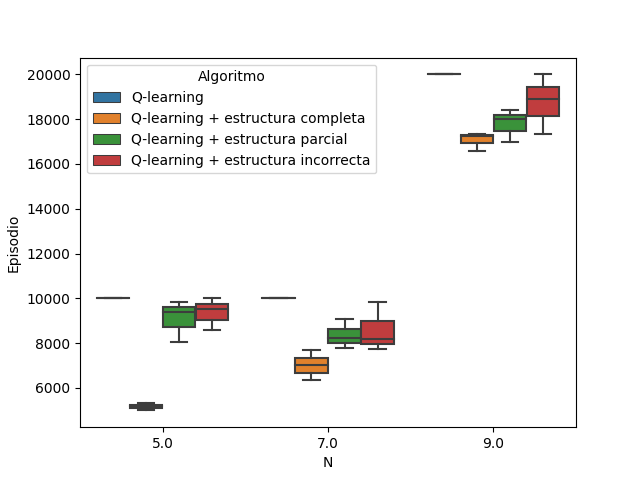
\includegraphics[width=0.5\textwidth]{Chapter5/Figs/modexp/boxplot_deterministic_one_to_one.png}\label{fig:boxplot-det-one-to-one}}
  \hfill
  \subfloat[Estructura uno a uno, ambiente estocástico.]{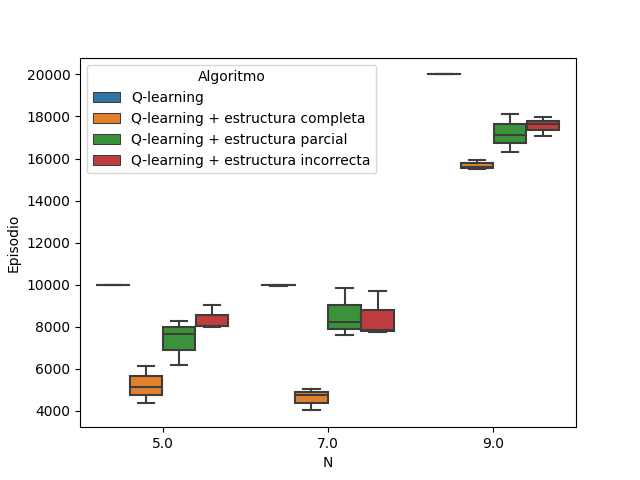
\includegraphics[width=0.5\textwidth]{Chapter5/Figs/modexp/boxplot_stochastic_one_to_one.png}\label{fig:boxplot-sto-one-to-one}}
  \\
  \subfloat[Estructura efecto común, ambiente determinista.]{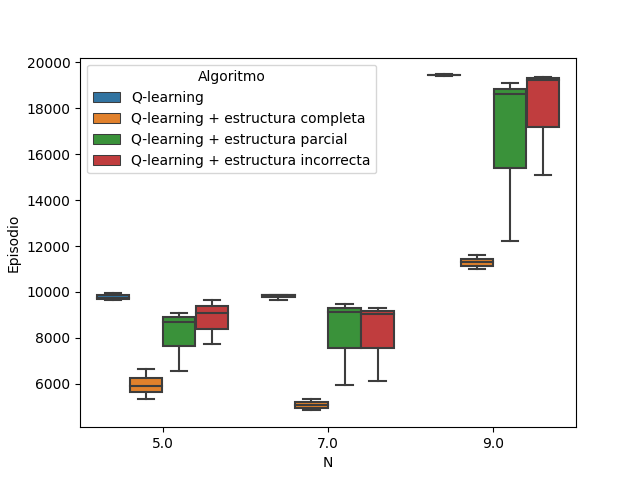
\includegraphics[width=0.5\textwidth]{Chapter5/Figs/modexp/boxplot_deterministic_many_to_one.png}\label{fig:boxplot-det-many-to-one}}
  \hfill
  \subfloat[Estructura efecto común, ambiente estocástico.]{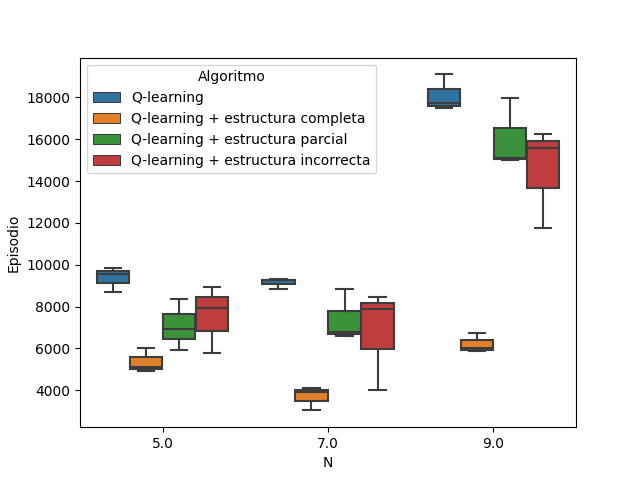
\includegraphics[width=0.5\textwidth]{Chapter5/Figs/modexp/boxplot_stochastic_many_to_one.png}\label{fig:boxplot-sto-many-to-one}}
  \\
  \subfloat[Estructura de causa común, ambiente determinista.]{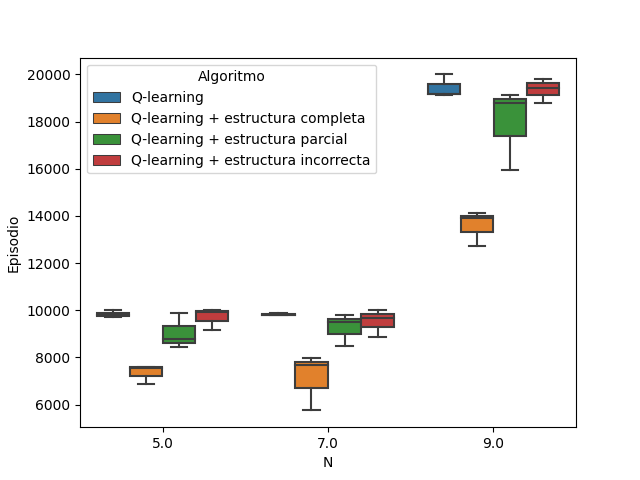
\includegraphics[width=0.5\textwidth]{Chapter5/Figs/modexp/boxplot_deterministic_one_to_many.png}\label{fig:boxplot-det-one-to-many}}
  \hfill
      \subfloat[Estructura de causa común, ambiente estocástico.]{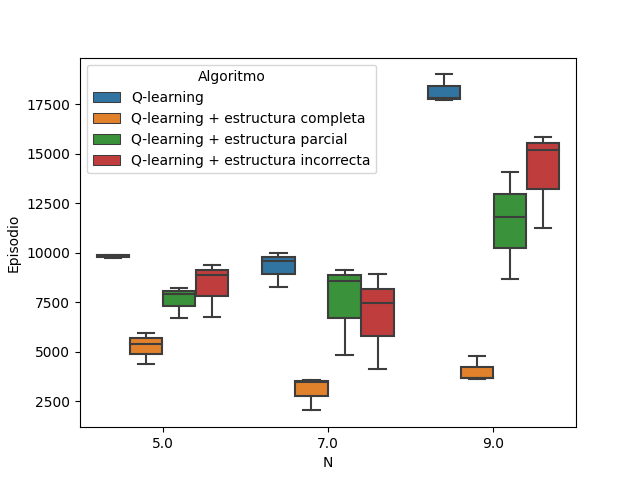
\includegraphics[width=0.5\textwidth]{Chapter5/Figs/modexp/boxplot_stochastic_one_to_many.png}\label{fig:boxplot-sto-one-to-many}}
      \caption{Diagramas de caja y bigote que resumen los resultados del desempeño de las diferentes configuraciones del experimento. El eje vertical describe el número de
      episodios en alcanzar la recompensa óptima y sobre el eje horizontal están los
      diferentes $N$ y algoritmos. }\label{fig:boxplots-pmod}
\end{figure}




%%%%%%%%%%%%%%%%%%%%%%%%%%%%%%%%%%%%%%%%%%%%55
% \newpage
% \begin{table}[h]
% \centering
% \caption{Comparación de la recompensa promedio obtenida durante los últimos $E=100$ episodios de entrenamiento para $M$ experimentos en tareas con estructuras causales uno a uno. En negritas se resaltan las recompensas promedio mayores con respecto al resto de los algoritmos en una configuración experimental dada.}
% \label{tab:pmo-one-to-one}
% \resizebox{\textwidth}{!}{%
% \begin{tabular}{@{}ccclll@{}}
% \toprule
% Ambiente & $p_{mod}$ & Algoritmo & \multicolumn{3}{c}{$N$} \\ \cmidrule(l){4-6} 
%  &  &  & \multicolumn{1}{c}{5} & \multicolumn{1}{c}{7} & \multicolumn{1}{c}{9} \\ \midrule
% Determinista & $25\%$ & $Q_{1}$ & $-2.2182 \pm 0.6336$ & $-4.2527 \pm 0.9449$ & $-6.4783 \pm 1.0360$ \\
%  &  & $Q_{2}$ & $\mathbf{-1.8956 \pm 0.5285}$ & $\mathbf{-3.4366 \pm 0.7290}$ & $-5.5112 \pm 1.0322$ \\
%  &  & $Q_{3}$ & $-1.9240 \pm 0.4748$ & $-3.5972 \pm 0.7493$ & $\mathbf{-5.2752 \pm 0.8429}$ \\
%  &  & $Q_{4}$ & $-1.9818 \pm 0.4810$ & $-3.5400 \pm 0.6413$ & $-5.6452 \pm 0.8337$ \\ \cmidrule(l){2-6} 
%  & $50\%$ & $Q_{1}$ & $-2.2628 \pm 0.5568$ & $-4.3893 \pm 0.9663$ & $-6.4983 \pm 1.1034$ \\
%  &  & $Q_{2}$ & $\mathbf{-1.9269 \pm 0.5063}$ & $\mathbf{-3.3805 \pm 0.6799}$ & $\mathbf{-5.3568 \pm 1.0327}$ \\
%  &  & $Q_{3}$ & $-2.0227 \pm 0.5103$ & $-3.6810 \pm 0.7031$ & $-5.5596 \pm 0.9284$ \\
%  &  & $Q_{4}$ & $-2.0515 \pm 0.5205$ & $-3.7771 \pm 0.8140$ & $-5.7934 \pm 1.0148$ \\ \cmidrule(l){2-6} 
%  & $75\%$ & $Q_{1}$ & $-2.3585 \pm 0.6444$ & $-4.3475 \pm 0.8879$ & $-6.4210 \pm 1.1059$ \\
%  &  & $Q_{2}$ & $\mathbf{-1.8609 \pm 0.4570}$ & $\mathbf{-3.4178 \pm 0.7382}$ & $\mathbf{-5.4319 \pm 0.9450}$ \\
%  &  & $Q_{3}$ & $-2.1248 \pm 0.5040$ & $-3.8530 \pm 0.8418$ & $-5.8715 \pm 1.0626$ \\
%  &  & $Q_{4}$ & $-2.1903 \pm 0.6093\dagger$ & $-4.0736 \pm 0.8175$ & $-6.2007 \pm 0.9860\dagger$ \\ \midrule
% Estocástico & $25\%$ & $Q_{1}$ & $-5.1114 \pm 0.9096$ & $-9.1281 \pm 1.1897$ & $-14.1541 \pm 1.5689$ \\
%  &  & $Q_{2}$ & $\mathbf{-3.7371 \pm 0.8183}$ & $\mathbf{-6.9731 \pm 1.2073}$ & $\mathbf{-9.6946 \pm 1.7353}$ \\
%  &  & $Q_{3}$ & $-3.8397 \pm 0.9062$ & $-7.4121 \pm 1.1744$ & $-11.2450 \pm 1.7928$ \\
%  &  & $Q_{4}$ & $-3.7755 \pm 0.7262$ & $-7.4194 \pm 1.3376$ & $-11.3526 \pm 1.9065$ \\ \cmidrule(l){2-6} 
%  & $50\%$ & $Q_{1}$ & $-4.8947 \pm 0.7977$ & $-9.2118 \pm 1.2497$ & $-13.8851 \pm 1.5869$ \\
%  &  & $Q_{2}$ & $\mathbf{-3.5493 \pm 0.8052}$ & $\mathbf{-7.3603 \pm 1.3592}$ & $\mathbf{-10.1254 \pm 1.8590}$ \\
%  &  & $Q_{3}$ & $-4.0995 \pm 0.8538$ & $-8.0543 \pm 1.2003$ & $-12.2734 \pm 1.5236$ \\
%  &  & $Q_{4}$ & $-4.0742 \pm 1.0099$ & $-7.8257 \pm 1.2826$ & $-11.9317 \pm 1.6780$ \\ \cmidrule(l){2-6} 
%  & $75\%$ & $Q_{1}$ & $-4.7275 \pm 0.8827$ & $-9.0077 \pm 1.1266$ & $-13.8726 \pm 1.5532$ \\
%  &  & $Q_{2}$ & $\mathbf{-3.4796 \pm 0.7879}$ & $\mathbf{-6.9571 \pm 1.4064}$ & $\mathbf{-9.8165 \pm 1.9188}$ \\
%  &  & $Q_{3}$ & $-4.2609 \pm 0.8242$ & $-8.5903 \pm 1.2043$ & $-12.5843 \pm 1.7400$ \\
%  &  & $Q_{4}$ & $-4.2405 \pm 0.9147$ & $-8.7413 \pm 1.4550\dagger$ & $-12.9938 \pm 1.4176$ \\ \bottomrule
% \end{tabular}%
% }
% \end{table}

% \newpage
% \begin{table}[h]
% \centering
% \caption{Comparación de la recompensa promedio obtenida durante los últimos $E=100$ episodios de entrenamiento para $M$ experimentos en tareas con estructuras causales del tipo causa común. En negritas se resaltan las recompensas promedio mayores con respecto al resto de los algoritmos en una configuración experimental dada.}
% \label{tab:pmo-many-to-one}
% \resizebox{\textwidth}{!}{%
% \begin{tabular}{@{}ccclll@{}}
% \toprule
% Ambiente & $p_{mod}$ & Algoritmo & \multicolumn{3}{c}{$N$} \\ \cmidrule(l){4-6} 
%  &  &  & \multicolumn{1}{c}{5} & \multicolumn{1}{c}{7} & \multicolumn{1}{c}{9} \\ \midrule
% Determinista & $25\%$ & $Q_{1}$ & $-1.1605 \pm 0.4370$ & $-2.3821 \pm 0.5554$ & $-3.6241 \pm 0.8354$ \\
%  &  & $Q_{2}$ & $\mathbf{-0.8818 \pm 0.2987}$ & $\mathbf{-1.8817 \pm 0.5535}$ & $\mathbf{-2.9917 \pm 0.6222}$ \\
%  &  & $Q_{3}$ & $-0.8999 \pm 0.3342$ & $-1.8906 \pm 0.5059$ & $-3.1555 \pm 0.7857$ \\
%  &  & $Q_{4}$ & $-0.9052 \pm 0.3063$ & $-1.9772 \pm 0.5410$ & $-3.1813 \pm 0.6925$ \\ \cmidrule(l){2-6} 
%  & $50\%$ & $Q_{1}$ & $-1.2611 \pm 0.4208$ & $-2.2211 \pm 0.6455$ & $-2.8791 \pm 0.7447$ \\
%  &  & $Q_{2}$ & $\mathbf{-0.9493 \pm 0.2981}$ & $\mathbf{-1.6838 \pm 0.4796}$ & $\mathbf{-2.2900 \pm 0.5628}$ \\
%  &  & $Q_{3}$ & $-1.0367 \pm 0.3289$ & $-1.8876 \pm 0.5945$ & $-2.4913 \pm 0.7249$ \\
%  &  & $Q_{4}$ & $-1.0658 \pm 0.4114$ & $-1.8973 \pm 0.5475$ & $-2.8104 \pm 0.7954\dagger$ \\ \cmidrule(l){2-6} 
%  & $75\%$ & $Q_{1}$ & $-1.3095 \pm 0.4857$ & $-2.4471 \pm 0.6858$ & $-3.7470 \pm 0.9684$ \\
%  &  & $Q_{2}$ & $\mathbf{-1.0618 \pm 0.3104}$ & $\mathbf{-1.9527 \pm 0.5322}$ & $\mathbf{-3.0603 \pm 0.6601}$ \\
%  &  & $Q_{3}$ & $-1.1391 \pm 0.3324$ & $-2.1410 \pm 0.5985$ & $-3.4041 \pm 0.8123$ \\
%  &  & $Q_{4}$ & $-1.2016 \pm 0.4291\dagger$ & $-2.4146 \pm 0.6697\dagger$ & $-3.5423 \pm 0.7628\dagger$ \\ \midrule
% Estocástico & $25\%$ & $Q_{1}$ & $-3.0886 \pm 0.9845$ & $-6.1796 \pm 1.6089$ & $-9.2795 \pm 2.0556$ \\
%  &  & $Q_{2}$ & $\mathbf{-2.1093 \pm 0.6978}$ & $\mathbf{-4.2816 \pm 1.1846}$ & $\mathbf{-5.2987 \pm 1.4281}$ \\
%  &  & $Q_{3}$ & $-2.2082 \pm 0.7754$ & $-4.4287 \pm 1.0685$ & $-5.6103 \pm 1.4823$ \\
%  &  & $Q_{4}$ & $-2.2333 \pm 0.7078$ & $-4.4320 \pm 1.2439$ & $-5.4898 \pm 1.5539$ \\ \cmidrule(l){2-6} 
%  & $50\%$ & $Q_{1}$ & $-2.9996 \pm 1.0511$ & $-6.0544 \pm 1.2444$ & $-8.4563 \pm 1.8175$ \\
%  &  & $Q_{2}$ & $\mathbf{-2.1329 \pm 0.7398}$ & $\mathbf{-4.1256 \pm 1.2303}$ & $\mathbf{-5.8154 \pm 1.4156}$ \\
%  &  & $Q_{3}$ & $-2.4228 \pm 0.7311$ & $-4.6498 \pm 1.1331$ & $-6.9922 \pm 1.6813$ \\
%  &  & $Q_{4}$ & $-2.4134 \pm 0.8149$ & $-4.1292 \pm 1.1034$ & $-6.5562 \pm 1.4675$ \\ \cmidrule(l){2-6} 
%  & $75\%$ & $Q_{1}$ & $-3.0753 \pm 0.8946$ & $-5.6907 \pm 1.3626$ & $-9.0473 \pm 2.0631$ \\
%  &  & $Q_{2}$ & $\mathbf{-2.1460 \pm 0.7327}$ & $\mathbf{-3.6353 \pm 1.1232}$ & $\mathbf{-5.3417 \pm 1.3045}$ \\
%  &  & $Q_{3}$ & $-2.2385 \pm 0.7288$ & $-4.8728 \pm 1.1800$ & $-6.3821 \pm 1.3441$ \\
%  &  & $Q_{4}$ & $-2.3781 \pm 0.8174$ & $-4.3506 \pm 1.2888$ & $-6.8824 \pm 1.8552$ \\ \bottomrule
% \end{tabular}%
% }
% \end{table}

% \newpage
% \begin{table}[h]
% \centering
% \caption{Comparación de la recompensa promedio obtenida durante los últimos $E=100$ episodios de entrenamiento para $M$ experimentos en tareas con estructuras causales de efecto común. En negritas se resaltan las recompensas promedio mayores con respecto al resto de los algoritmos en una configuración experimental dada.}
% \label{tab:pmo-one-to-many}
% \resizebox{\textwidth}{!}{%
% \begin{tabular}{@{}ccclll@{}}
% \toprule
% Ambiente & $p_{mod}$ & Algoritmo & \multicolumn{3}{c}{$N$} \\ \cmidrule(l){4-6} 
%  &  &  & \multicolumn{1}{c}{5} & \multicolumn{1}{c}{7} & \multicolumn{1}{c}{9} \\ \midrule
% Determinista & $25\%$ & $Q_{1}$ & $-1.1566 \pm 0.4032$ & $-2.0655 \pm 0.5925$ & $-2.5841 \pm 0.6171$ \\
%  &  & $Q_{2}$ & $\mathbf{-0.9035 \pm 0.2978}$ & $\mathbf{-1.6037 \pm 0.4009}$ & $\mathbf{-2.1047 \pm 0.5454}$ \\
%  &  & $Q_{3}$ & $-0.9295 \pm 0.3044$ & $-1.6527 \pm 0.5065$ & $-2.1139 \pm 0.5718$ \\
%  &  & $Q_{4}$ & $-0.9903 \pm 0.3278$ & $-1.6576 \pm 0.4356$ & $-2.3156 \pm 0.5591$ \\ \cmidrule(l){2-6} 
%  & $50\%$ & $Q_{1}$ & $-1.1123 \pm 0.4498$ & $-2.0584 \pm 0.6533$ & $-2.9029 \pm 0.7290$ \\
%  &  & $Q_{2}$ & $\mathbf{-0.8622 \pm 0.2878}$ & $\mathbf{-1.6729 \pm 0.4784}$ & $\mathbf{-2.3992 \pm 0.5821}$ \\
%  &  & $Q_{3}$ & $-0.9735 \pm 0.3656$ & $-1.8843 \pm 0.4881$ & $-2.5665 \pm 0.5631$ \\
%  &  & $Q_{4}$ & $-1.0127 \pm 0.3423\dagger$ & $-2.0133 \pm 0.5224\dagger$ & $-2.6393 \pm 0.7003$ \\ \cmidrule(l){2-6} 
%  & $75\%$ & $Q_{1}$ & $-0.9944 \pm 0.3483$ & $-2.3420 \pm 0.6175$ & $-3.2112 \pm 0.7041$ \\
%  &  & $Q_{2}$ & $\mathbf{-0.7371 \pm 0.2555}$ & $\mathbf{-1.8766 \pm 0.4679}$ & $\mathbf{-2.5704 \pm 0.5597}$ \\
%  &  & $Q_{3}$ & $-0.8670 \pm 0.3424$ & $-2.1462 \pm 0.5880$ & $-2.8315 \pm 0.6618$ \\
%  &  & $Q_{4}$ & $-0.8988 \pm 0.3557\dagger$ & $-2.2513 \pm 0.5743\dagger$ & $-3.0330 \pm 0.6829\dagger$ \\ \midrule
% Estocástico & $25\%$ & $Q_{1}$ & $-2.4246 \pm 0.7587$ & $-4.9754 \pm 1.2124$ & $-7.7349 \pm 1.4403$ \\
%  &  & $Q_{2}$ & $\mathbf{-1.6373 \pm 0.6081}$ & $-3.5762 \pm 1.0292$ & $\mathbf{-4.8947 \pm 1.4667}$ \\
%  &  & $Q_{3}$ & $-1.8670 \pm 0.6335$ & $-3.6253 \pm 1.0470$ & $-5.6975 \pm 1.3601$ \\
%  &  & $Q_{4}$ & $-1.8538 \pm 0.5879$ & $\mathbf{-3.5423 \pm 0.9738}$ & $-4.9075 \pm 1.3517$ \\ \cmidrule(l){2-6} 
%  & $50\%$ & $Q_{1}$ & $-2.3026 \pm 0.6698$ & $-5.0139 \pm 1.0946$ & $-7.8808 \pm 1.3351$ \\
%  &  & $Q_{2}$ & $\mathbf{-1.4379 \pm 0.4905}$ & $-3.3055 \pm 0.9801$ & $\mathbf{-5.4403 \pm 1.3450}$ \\
%  &  & $Q_{3}$ & $-1.6029 \pm 0.5111$ & $-3.4351 \pm 0.9925$ & $-5.9440 \pm 1.4399$ \\
%  &  & $Q_{4}$ & $-1.7097 \pm 0.6777$ & $\mathbf{-3.2720 \pm 0.9536}$ & $-6.5544 \pm 1.4985$ \\ \cmidrule(l){2-6} 
%  & $75\%$ & $Q_{1}$ & $-2.3648 \pm 0.7404$ & $-5.1371 \pm 1.1200$ & $-7.6762 \pm 1.5876$ \\
%  &  & $Q_{2}$ & $\mathbf{-1.7755 \pm 0.5862}$ & $\mathbf{-3.2939 \pm 0.9156}$ & $\mathbf{-4.9183 \pm 1.2352}$ \\
%  &  & $Q_{3}$ & $-2.2238 \pm 0.6873\dagger$ & $-4.2950 \pm 1.1680$ & $-6.2311 \pm 1.5134$ \\
%  &  & $Q_{4}$ & $-2.1695 \pm 0.6820\dagger$ & $-4.1598 \pm 1.0756$ & $-6.1031 \pm 1.3614$ \\ \bottomrule
% \end{tabular}%
% }
% \end{table}

%%%%%%%%%%%%%%%%%
%%%PMOD 25 DET%%%
%%%%%%%%%%%%%%%%%
\begin{figure}
\settoheight{\tempdima}{\includegraphics[width=.32\linewidth]{example-image-a}}%
\centering\begin{tabular}{@{}c@{ }c@{ }c@{ }c@{}}
&\textbf{Uno-a-uno} & \textbf{Causa común} & \textbf{Efecto común} \\
\rowname{$N = 5$}&
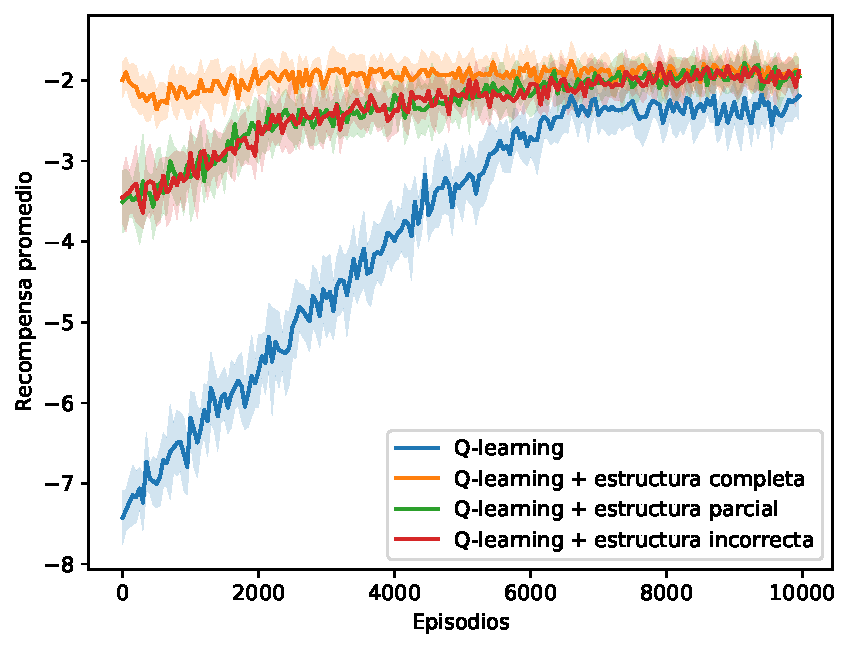
\includegraphics[width=.32\linewidth]{Chapter5/Figs/modexp/deterministic_low_025_one_to_one_N_5_experiments_10_episodes_10000_eps_25000.pdf}&
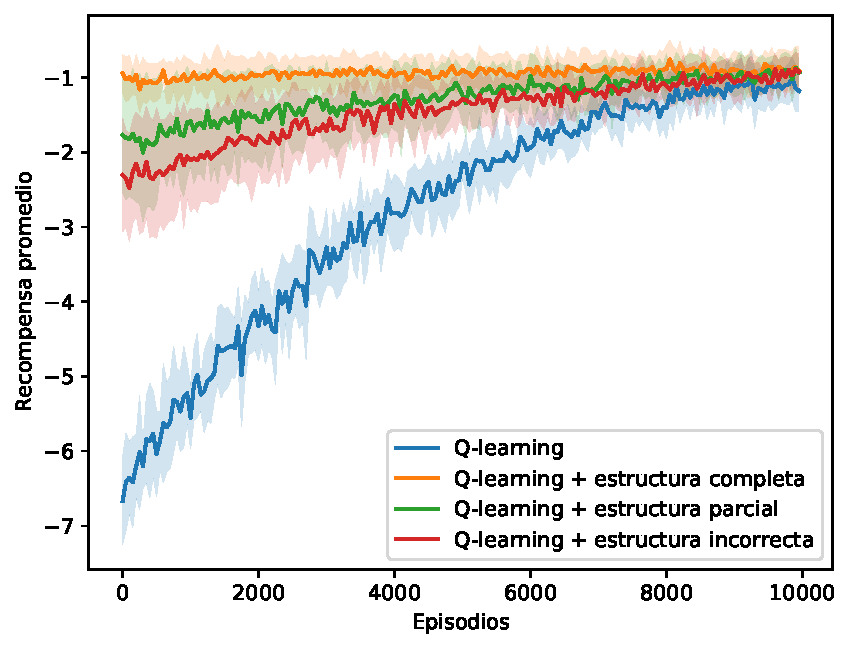
\includegraphics[width=.32\linewidth]{Chapter5/Figs/modexp/deterministic_low_025_one_to_many_N_5_experiments_10_episodes_10000_eps_25000.pdf}&
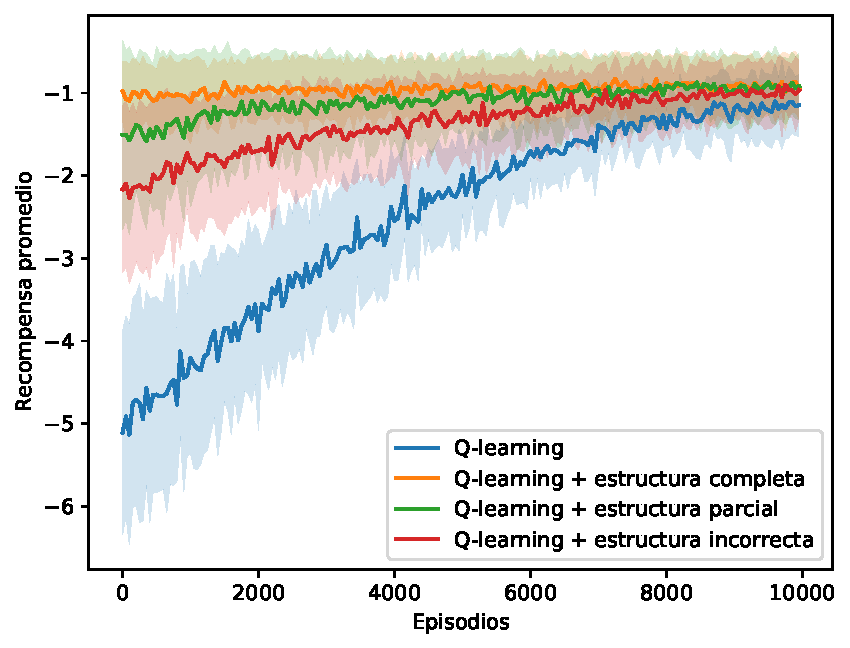
\includegraphics[width=.32\linewidth]{Chapter5/Figs/modexp/deterministic_low_025_many_to_one_N_5_experiments_10_episodes_10000_eps_25000.pdf}
\\
\rowname{$N=7$}&
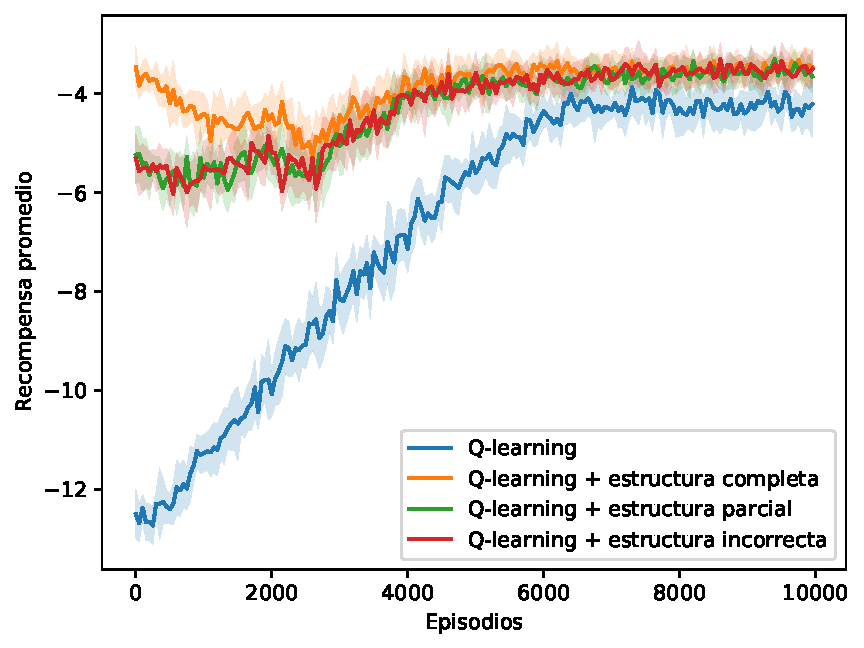
\includegraphics[width=.32\linewidth]{Chapter5/Figs/modexp/deterministic_low_025_one_to_one_N_7_experiments_10_episodes_10000_eps_35000.pdf}&
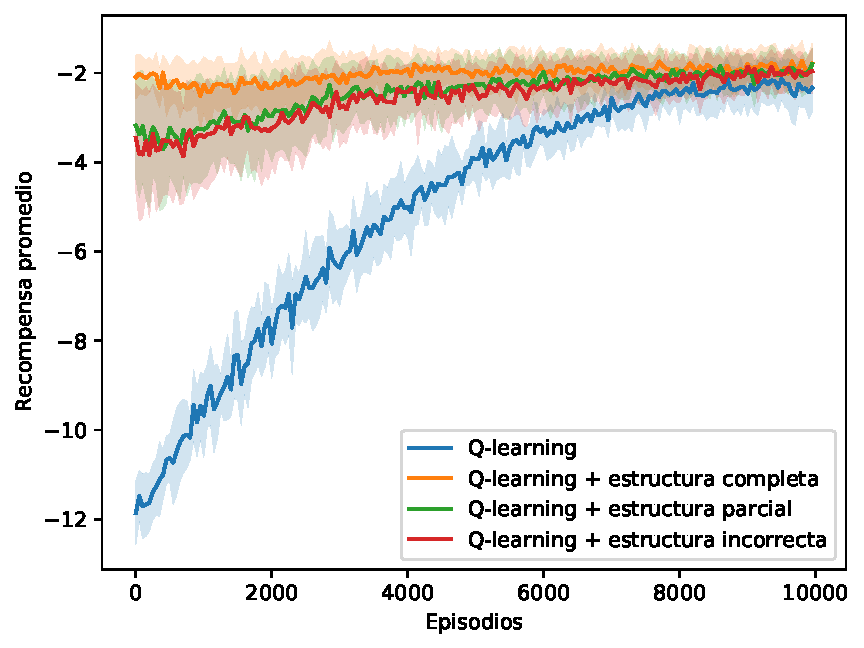
\includegraphics[width=.32\linewidth]{Chapter5/Figs/modexp/deterministic_low_025_one_to_many_N_7_experiments_10_episodes_10000_eps_35000.pdf}&
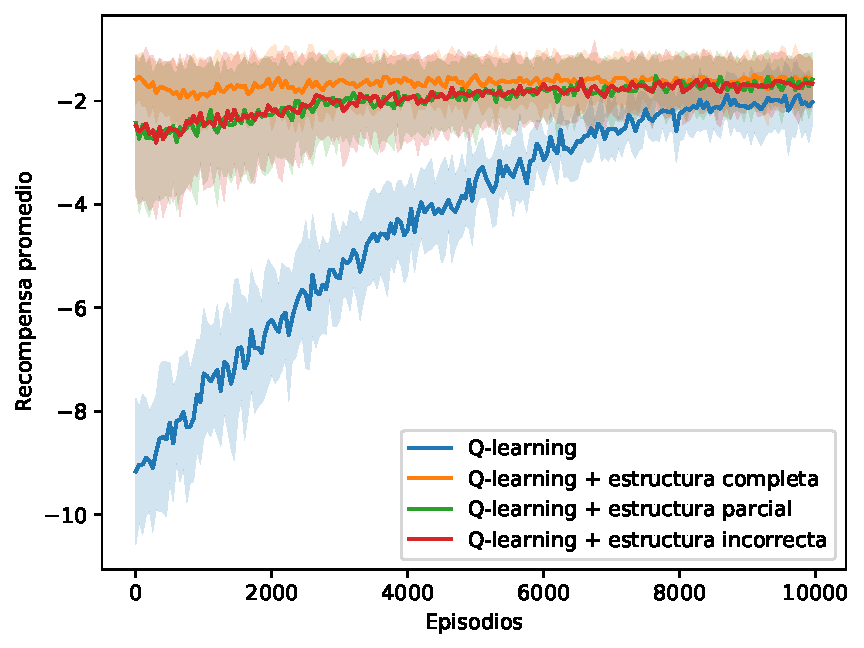
\includegraphics[width=.32\linewidth]{Chapter5/Figs/modexp/deterministic_low_025_many_to_one_N_7_experiments_10_episodes_10000_eps_35000.pdf}
\\
\rowname{$N = 9$}&

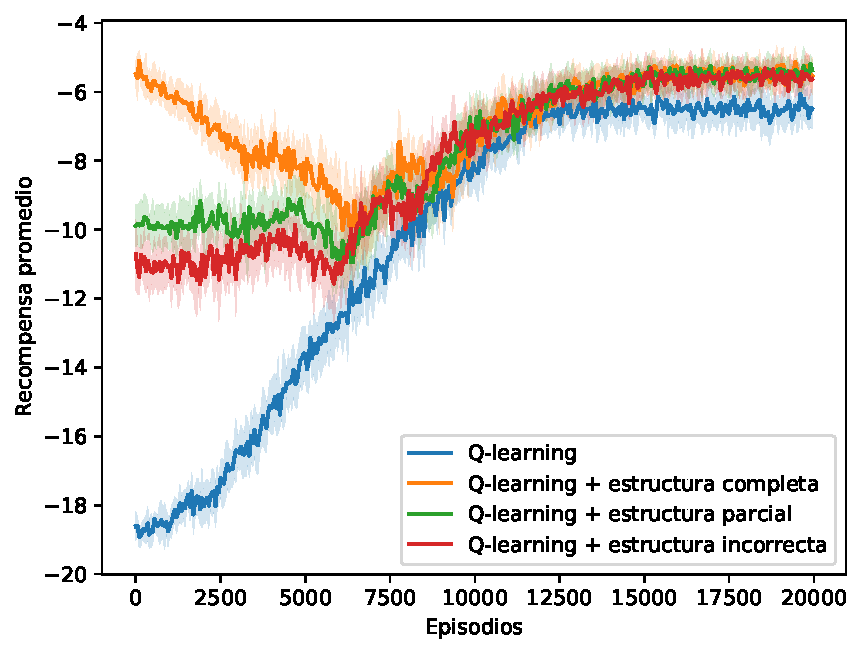
\includegraphics[width=.32\linewidth]{Chapter5/Figs/modexp/deterministic_low_025_one_to_one_N_9_experiments_10_episodes_20000_eps_90000.pdf}&
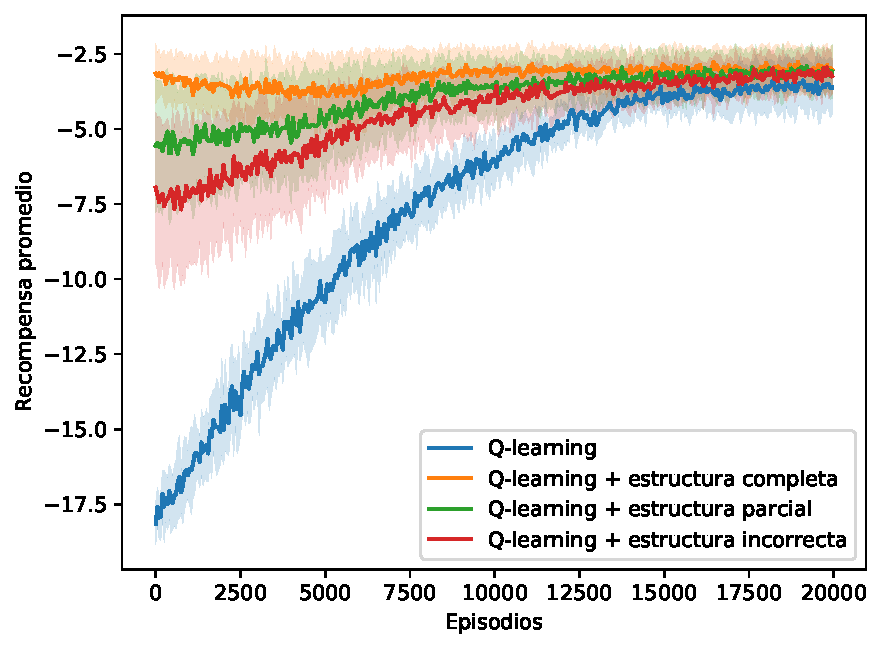
\includegraphics[width=.32\linewidth]{Chapter5/Figs/modexp/deterministic_low_025_one_to_many_N_9_experiments_10_episodes_20000_eps_90000.pdf}&
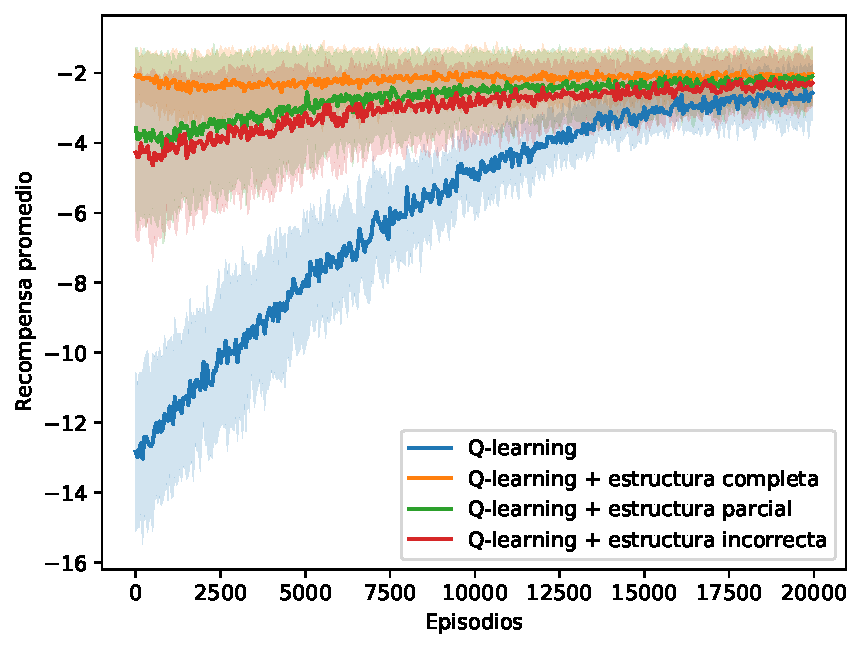
\includegraphics[width=.32\linewidth]{Chapter5/Figs/modexp/deterministic_low_025_many_to_one_N_9_experiments_10_episodes_20000_eps_90000.pdf}

\end{tabular}
\caption{Comparación del desempeño para los 4 algoritmos con un nivel de alteración $p_{mod} = 25 \%$ en un ambiente determinista. Las gráficas muestran la medida $average$ y la desviación estándar (región sombreada) para 10 experimentos con 10000 (para $N = 5, 7$) y 20000 (para $N = 9$) episodios.}
\label{fig:low-mod-det}
\end{figure}

%%%%%%%%%%%%%%%%%
%%%PMOD 25 STO%%%
%%%%%%%%%%%%%%%%%
\begin{figure}
\settoheight{\tempdima}{\includegraphics[width=.32\linewidth]{example-image-a}}%
\centering\begin{tabular}{@{}c@{ }c@{ }c@{ }c@{}}
&\textbf{Uno-a-uno} & \textbf{Causa común} & \textbf{Efecto común} \\
\rowname{$N = 5$}&
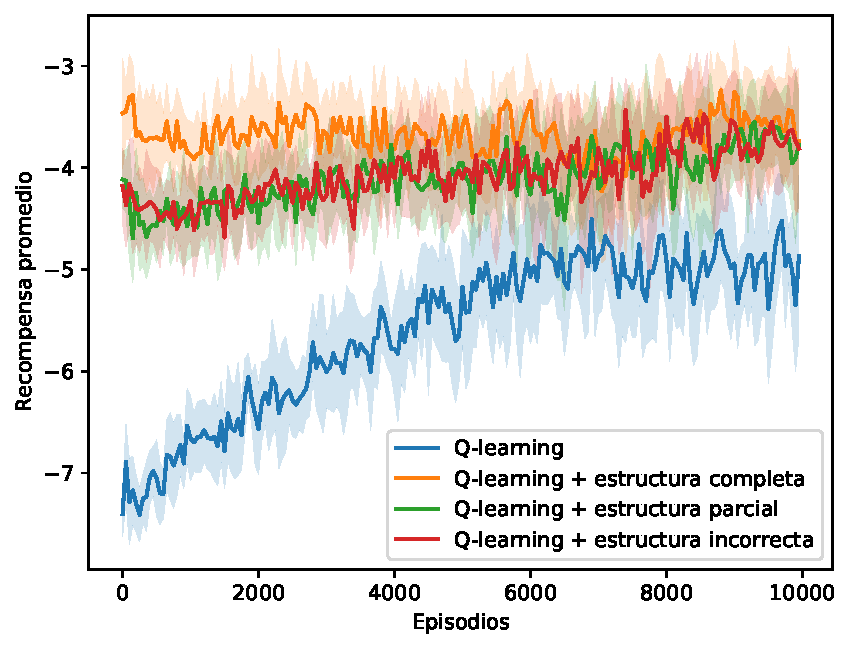
\includegraphics[width=.32\linewidth]{Chapter5/Figs/modexp/stochastic_low_025_one_to_one_N_5_experiments_10_episodes_10000_eps_25000.pdf}&
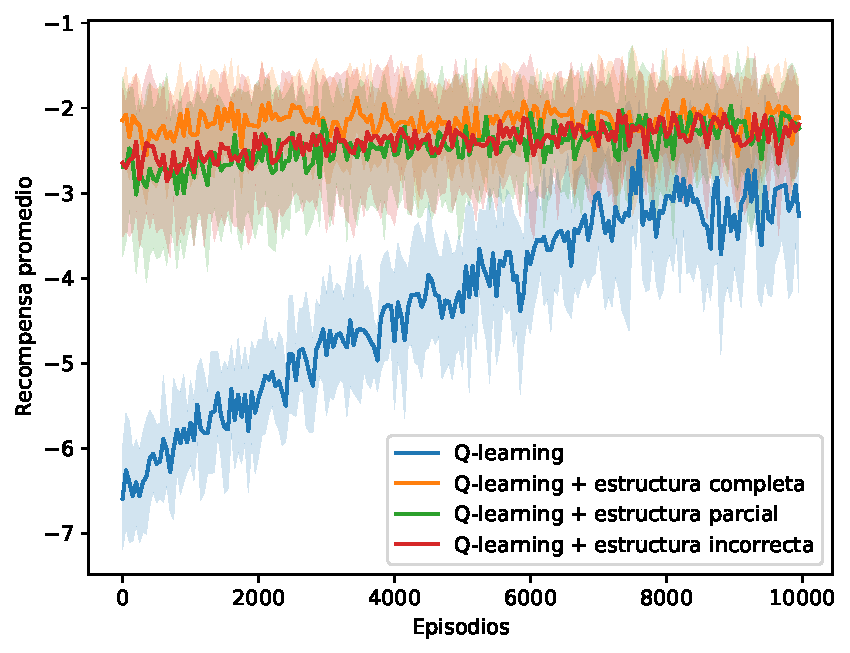
\includegraphics[width=.32\linewidth]{Chapter5/Figs/modexp/stochastic_low_025_one_to_many_N_5_experiments_10_episodes_10000_eps_25000.pdf}&
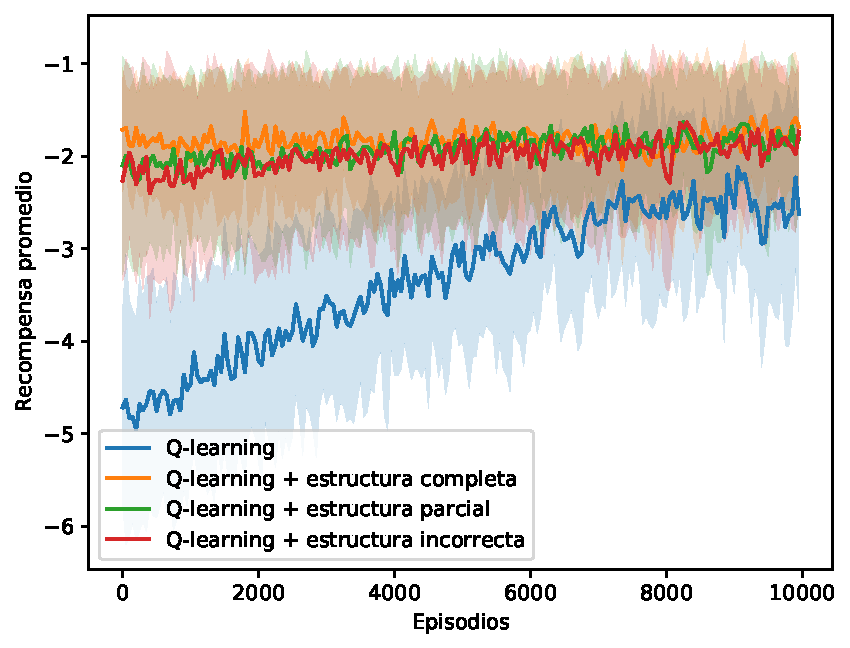
\includegraphics[width=.32\linewidth]{Chapter5/Figs/modexp/stochastic_low_025_many_to_one_N_5_experiments_10_episodes_10000_eps_25000.pdf}
\\
\rowname{$N=7$}&
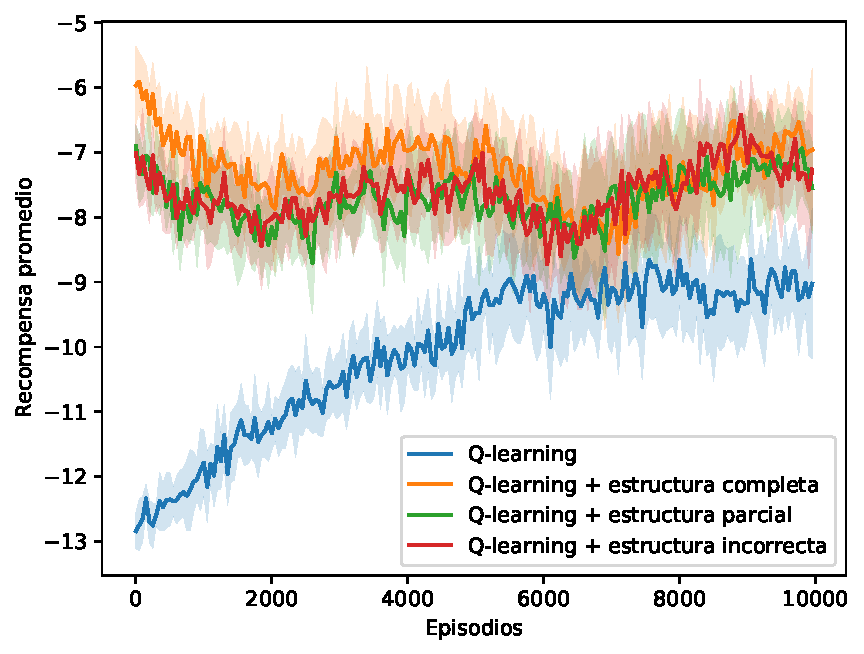
\includegraphics[width=.32\linewidth]{Chapter5/Figs/modexp/stochastic_low_025_one_to_one_N_7_experiments_10_episodes_10000_eps_35000.pdf}&
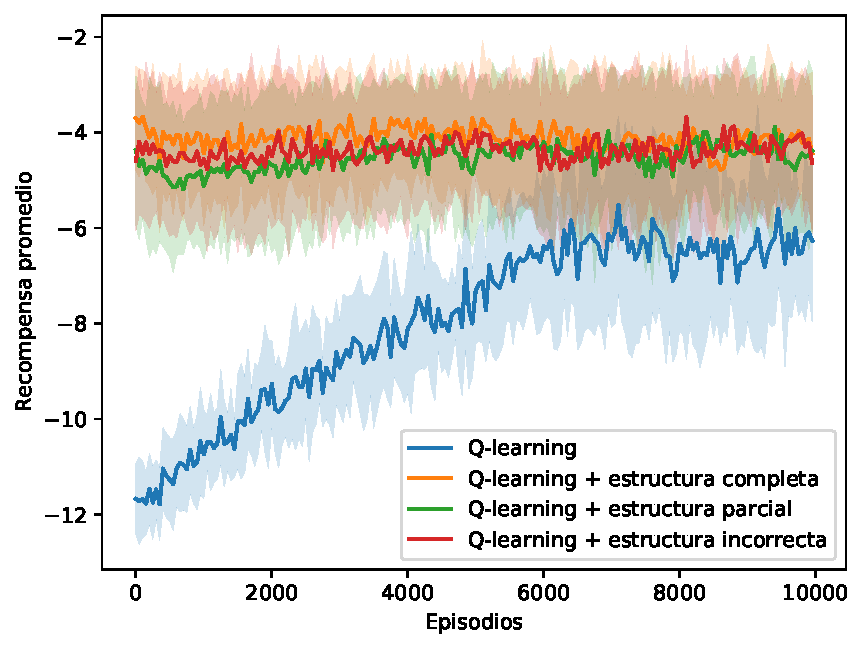
\includegraphics[width=.32\linewidth]{Chapter5/Figs/modexp/stochastic_low_025_one_to_many_N_7_experiments_10_episodes_10000_eps_35000.pdf}&
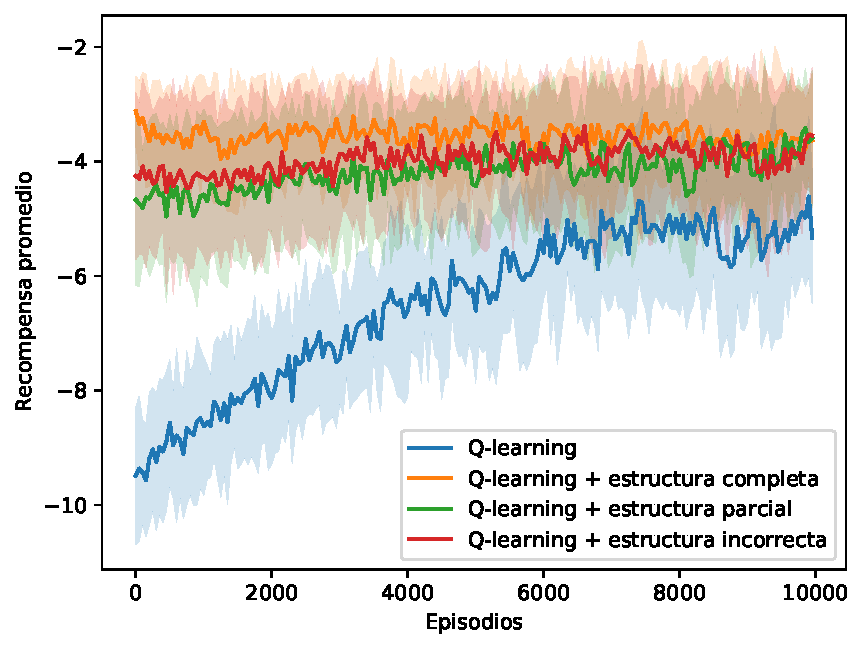
\includegraphics[width=.32\linewidth]{Chapter5/Figs/modexp/stochastic_low_025_many_to_one_N_7_experiments_10_episodes_10000_eps_35000.pdf}
\\
\rowname{$N = 9$}&

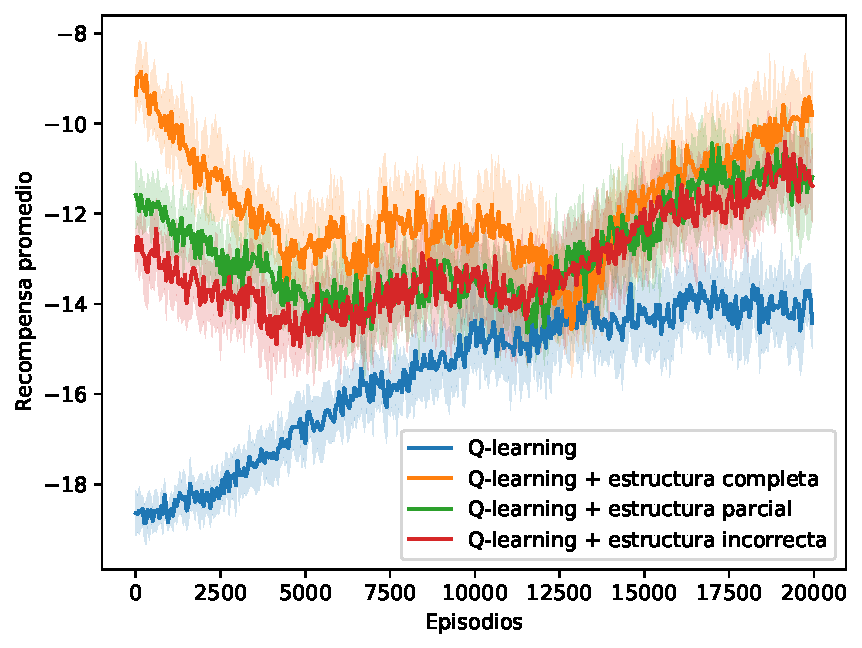
\includegraphics[width=.32\linewidth]{Chapter5/Figs/modexp/stochastic_low_025_one_to_one_N_9_experiments_10_episodes_20000_eps_90000.pdf}&
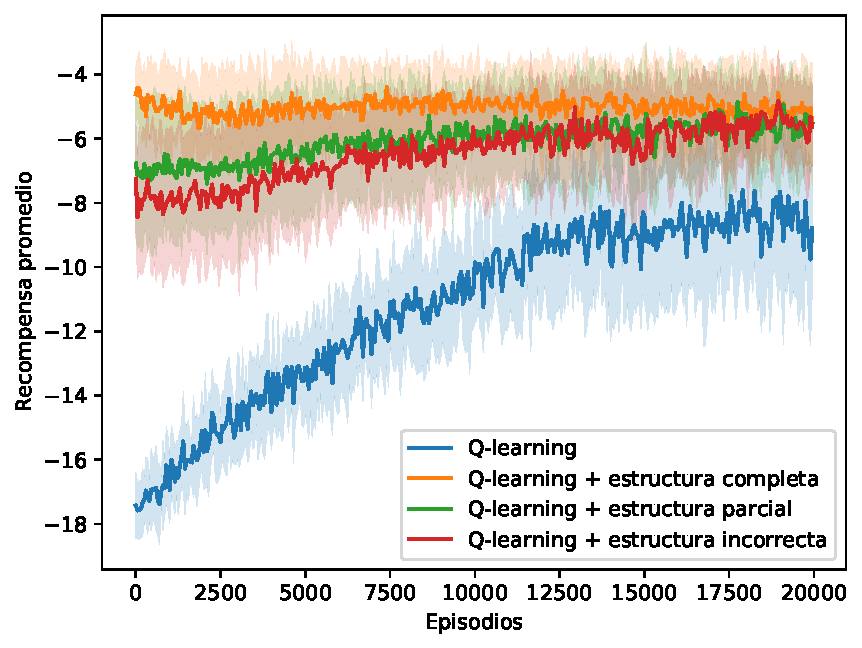
\includegraphics[width=.32\linewidth]{Chapter5/Figs/modexp/stochastic_low_025_one_to_many_N_9_experiments_10_episodes_20000_eps_90000.pdf}&
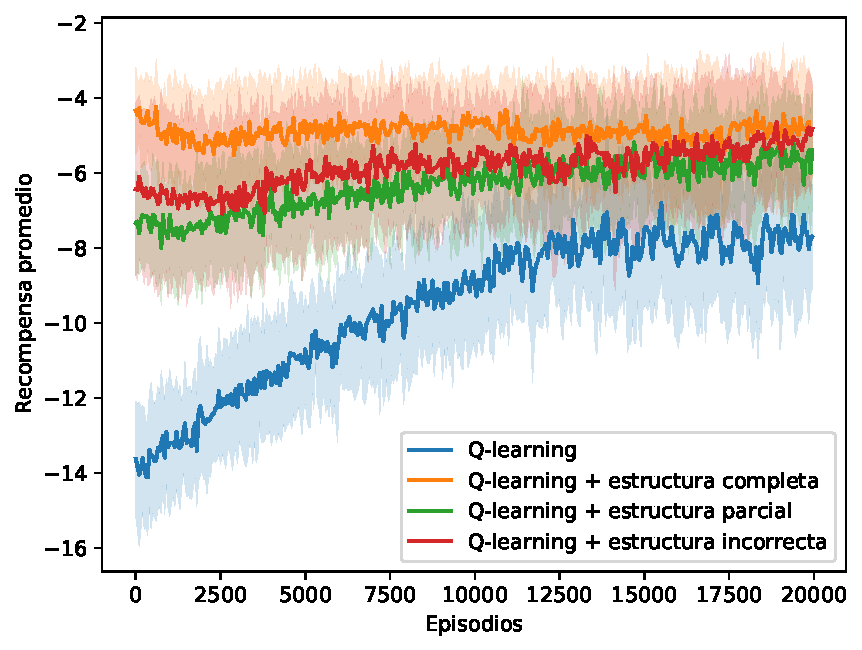
\includegraphics[width=.32\linewidth]{Chapter5/Figs/modexp/stochastic_low_025_many_to_one_N_9_experiments_10_episodes_20000_eps_90000.pdf}

\end{tabular}
\caption{Comparación del desempeño para los 4 algoritmos con un nivel de alteración $p_{mod} = 25 \%$ en un ambiente estocástico. Las gráficas muestran la medida $average$ y la desviación estándar (región sombreada) para 10 experimentos con 10000 (para $N = 5, 7$) y 20000 (para $N = 9$) episodios.}
\label{fig:low-mod-sto}
\end{figure}


\begin{figure}
\settoheight{\tempdima}{\includegraphics[width=.32\linewidth]{example-image-a}}%
\centering\begin{tabular}{@{}c@{ }c@{ }c@{ }c@{}}
&\textbf{Uno-a-uno} & \textbf{Causa común} & \textbf{Efecto común} \\
\rowname{$N = 5$}&
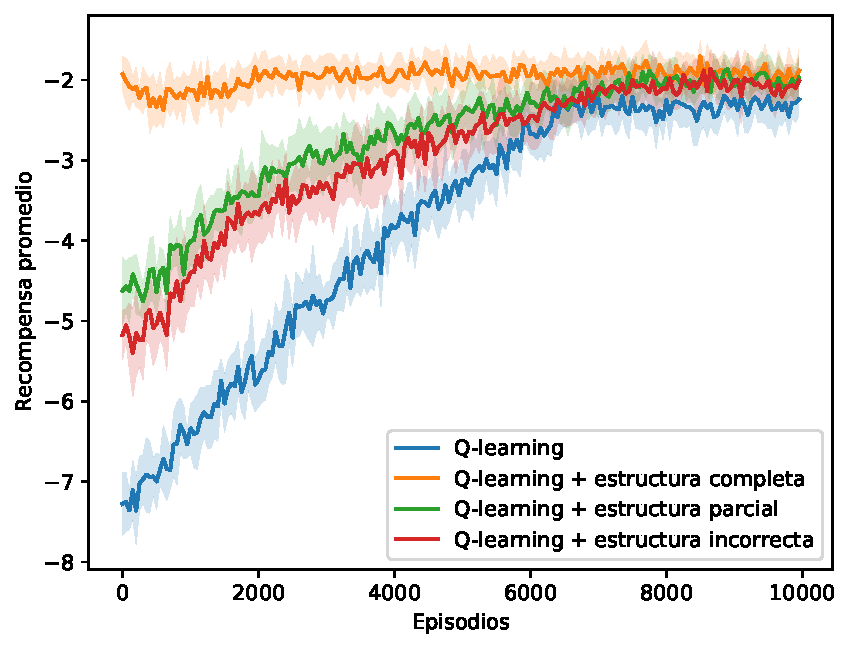
\includegraphics[width=.32\linewidth]{Chapter5/Figs/modexp/deterministic_medium_05_one_to_one_N_5_experiments_10_episodes_10000_eps_25000.pdf}&
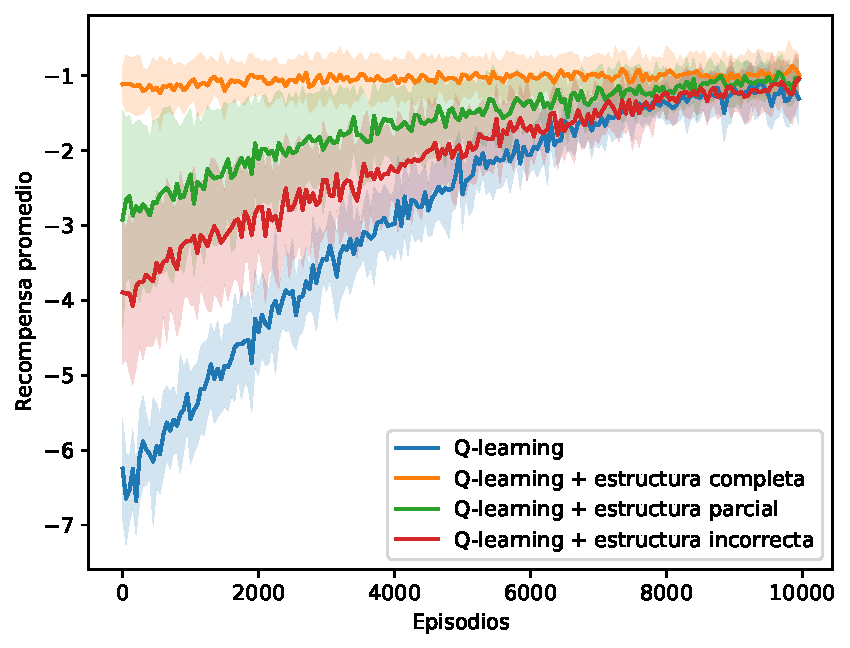
\includegraphics[width=.32\linewidth]{Chapter5/Figs/modexp/deterministic_medium_05_one_to_many_N_5_experiments_10_episodes_10000_eps_25000.pdf}&
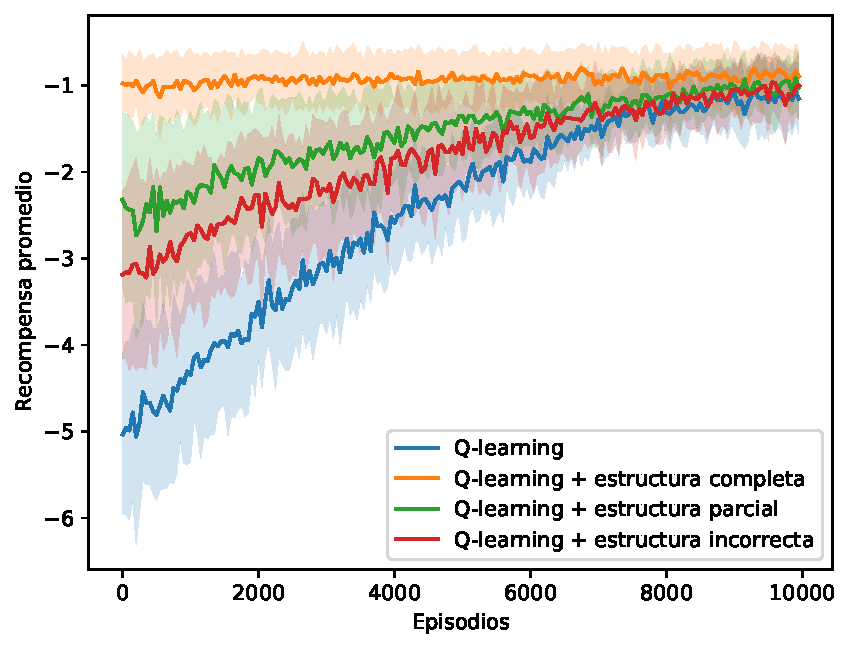
\includegraphics[width=.32\linewidth]{Chapter5/Figs/modexp/deterministic_medium_05_many_to_one_N_5_experiments_10_episodes_10000_eps_25000.pdf}
\\
\rowname{$N=7$}&
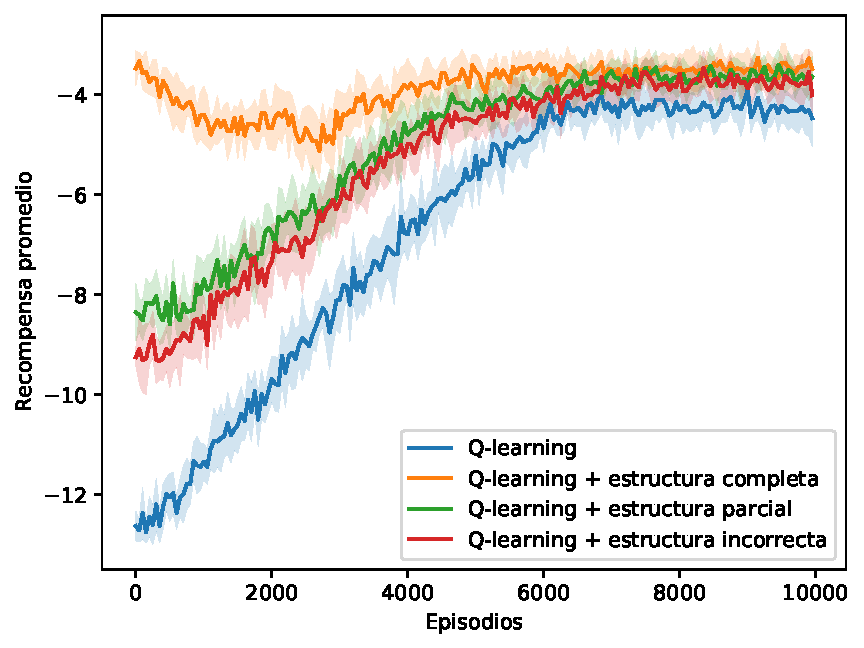
\includegraphics[width=.32\linewidth]{Chapter5/Figs/modexp/deterministic_medium_05_one_to_one_N_7_experiments_10_episodes_10000_eps_35000.pdf}&
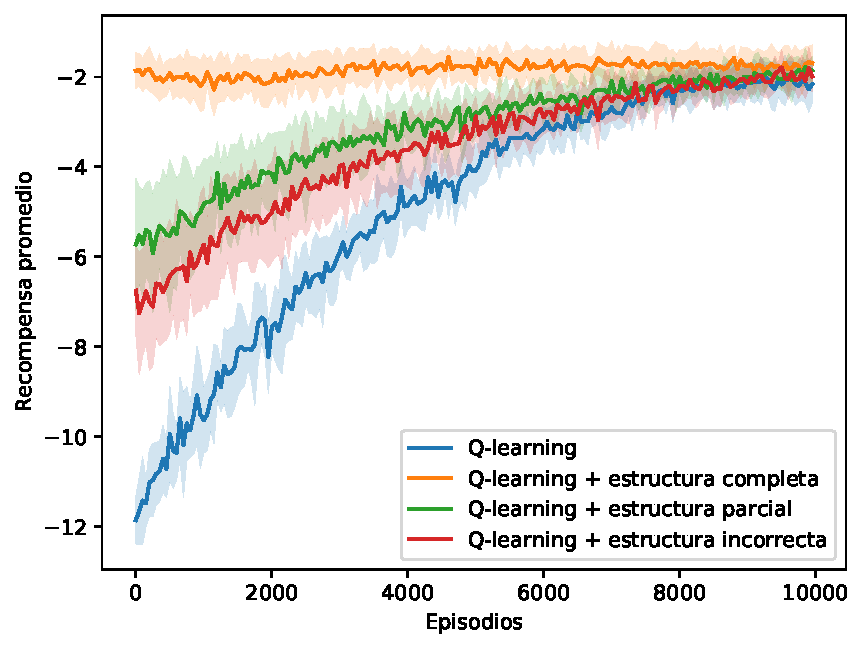
\includegraphics[width=.32\linewidth]{Chapter5/Figs/modexp/deterministic_medium_05_one_to_many_N_7_experiments_10_episodes_10000_eps_35000.pdf}&
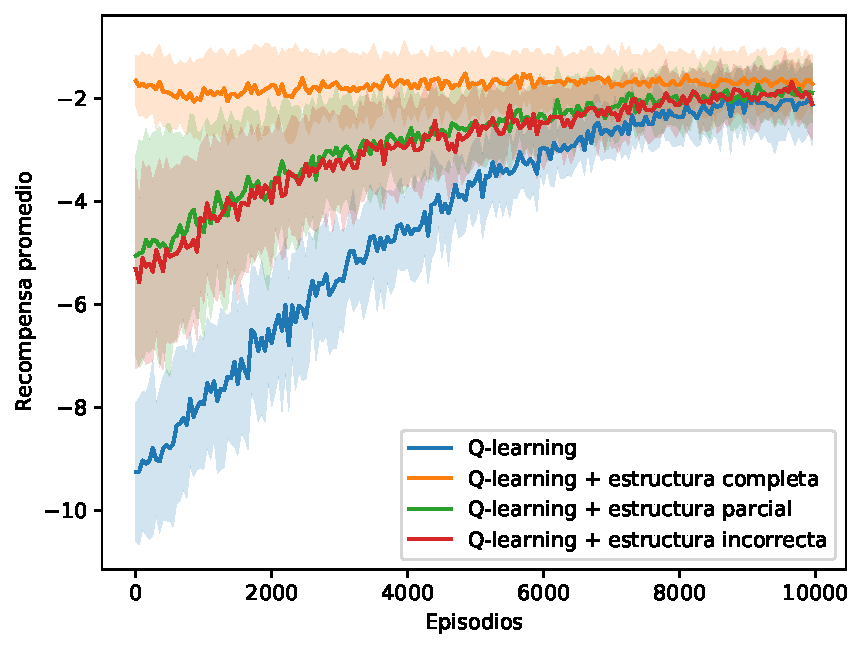
\includegraphics[width=.32\linewidth]{Chapter5/Figs/modexp/deterministic_medium_05_many_to_one_N_7_experiments_10_episodes_10000_eps_35000.pdf}
\\
\rowname{$N = 9$}&

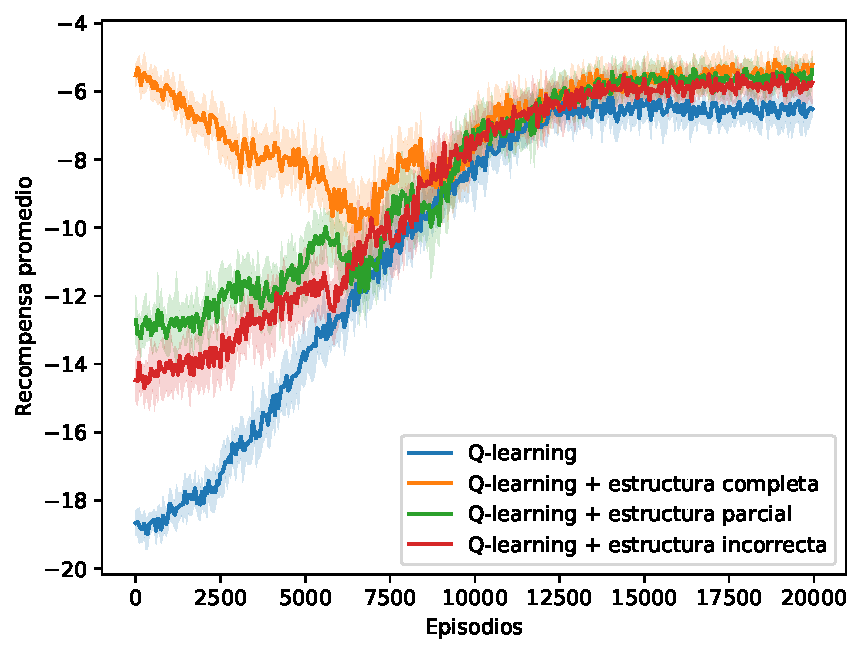
\includegraphics[width=.32\linewidth]{Chapter5/Figs/modexp/deterministic_medium_05_one_to_one_N_9_experiments_10_episodes_20000_eps_90000.pdf}&
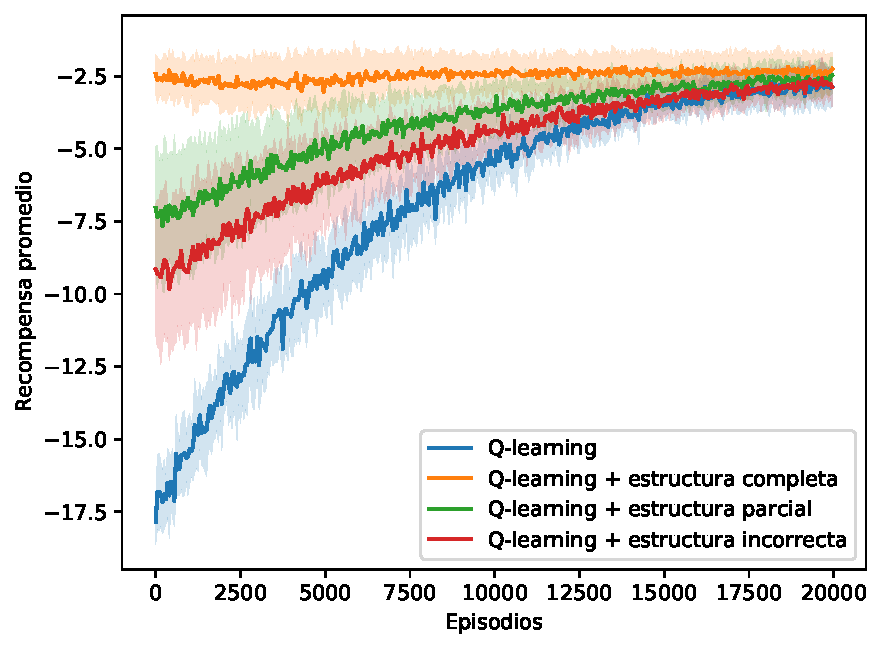
\includegraphics[width=.32\linewidth]{Chapter5/Figs/modexp/deterministic_medium_05_one_to_many_N_9_experiments_10_episodes_20000_eps_90000.pdf}&
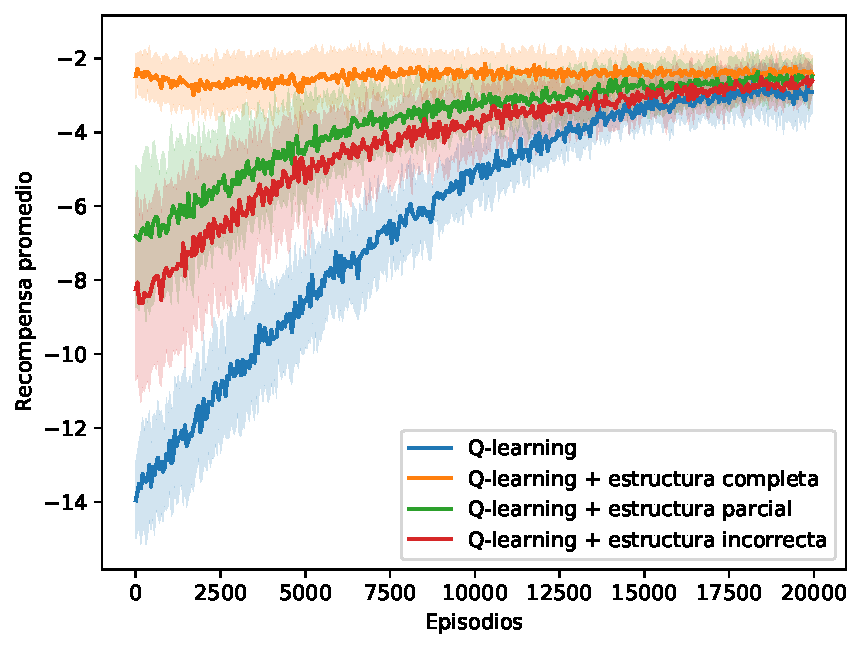
\includegraphics[width=.32\linewidth]{Chapter5/Figs/modexp/deterministic_medium_05_many_to_one_N_9_experiments_10_episodes_20000_eps_90000.pdf}

\end{tabular}
\caption{Comparación del desempeño para los 4 algoritmos con un nivel de alteración $p_{mod} = 50 \%$ en un ambiente determinista. Las gráficas muestran la medida $average$ y la desviación estándar (región sombreada)para 10 experimentos con 10000 (para $N = 5, 7$) y 20000 (para $N = 9$) episodios.}
\label{fig:med-mod-det}
\end{figure}



\begin{figure}
\settoheight{\tempdima}{\includegraphics[width=.32\linewidth]{example-image-a}}%
\centering\begin{tabular}{@{}c@{ }c@{ }c@{ }c@{}}
&\textbf{Uno-a-uno} & \textbf{Causa común} & \textbf{Efecto común} \\
\rowname{$N = 5$}&
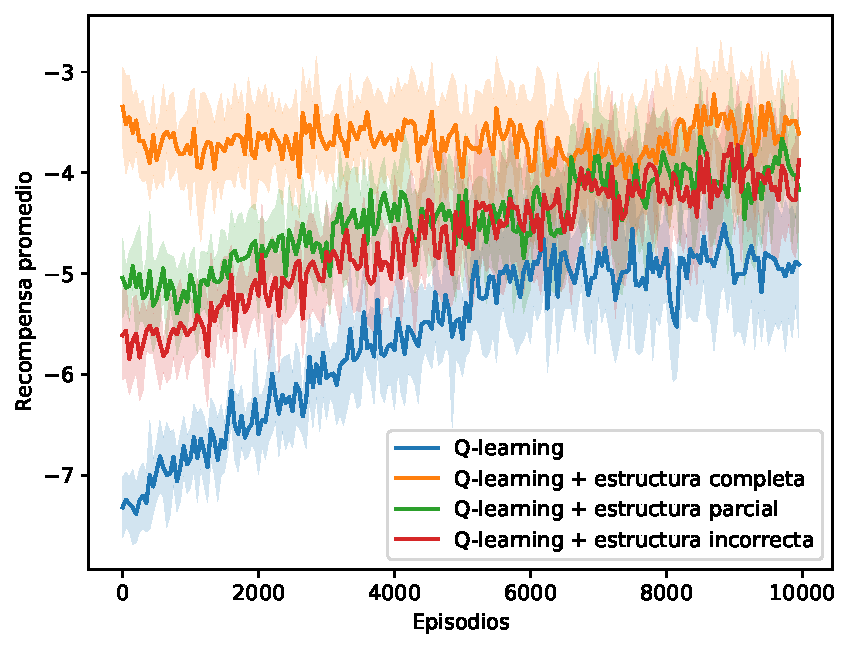
\includegraphics[width=.32\linewidth]{Chapter5/Figs/modexp/stochastic_medium_05_one_to_one_N_5_experiments_10_episodes_10000_eps_25000.pdf}&
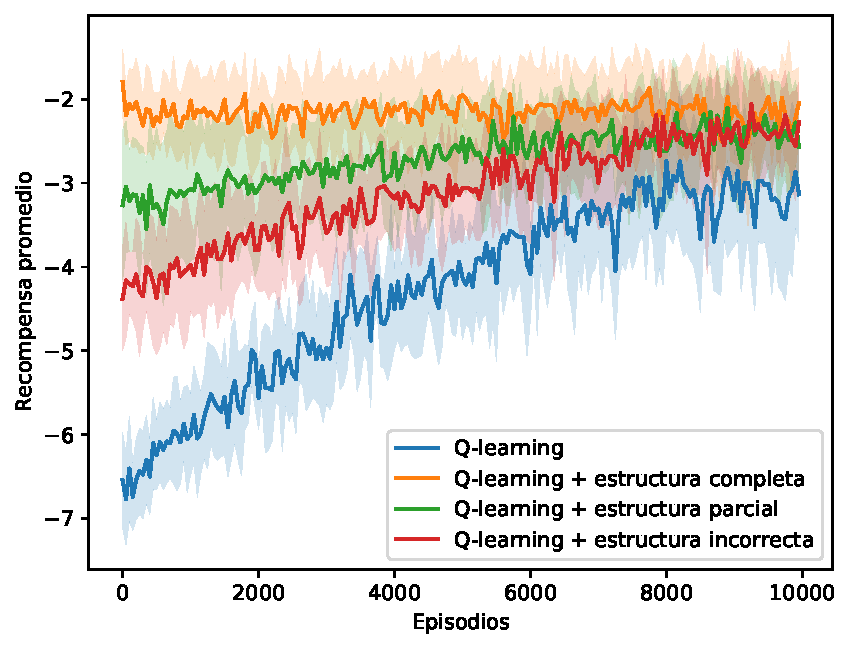
\includegraphics[width=.32\linewidth]{Chapter5/Figs/modexp/stochastic_medium_05_one_to_many_N_5_experiments_10_episodes_10000_eps_25000.pdf}&
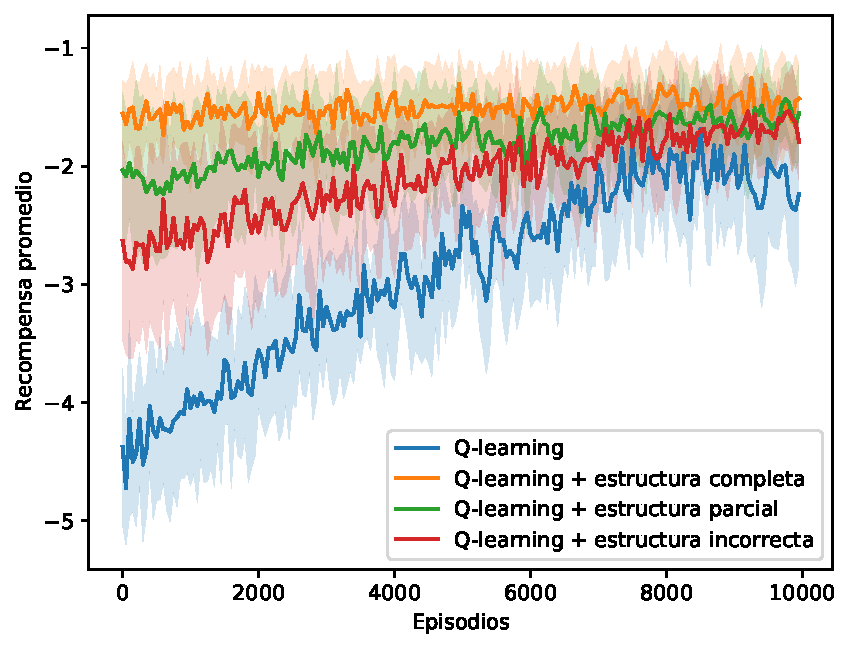
\includegraphics[width=.32\linewidth]{Chapter5/Figs/modexp/stochastic_medium_05_many_to_one_N_5_experiments_10_episodes_10000_eps_25000.pdf}
\\
\rowname{$N=7$}&
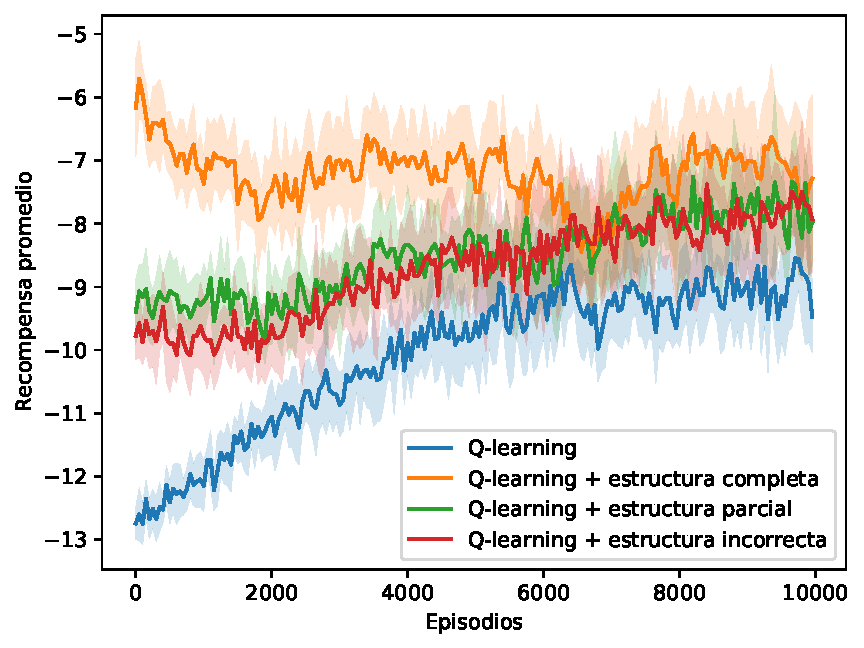
\includegraphics[width=.32\linewidth]{Chapter5/Figs/modexp/stochastic_medium_05_one_to_one_N_7_experiments_10_episodes_10000_eps_35000.pdf}&
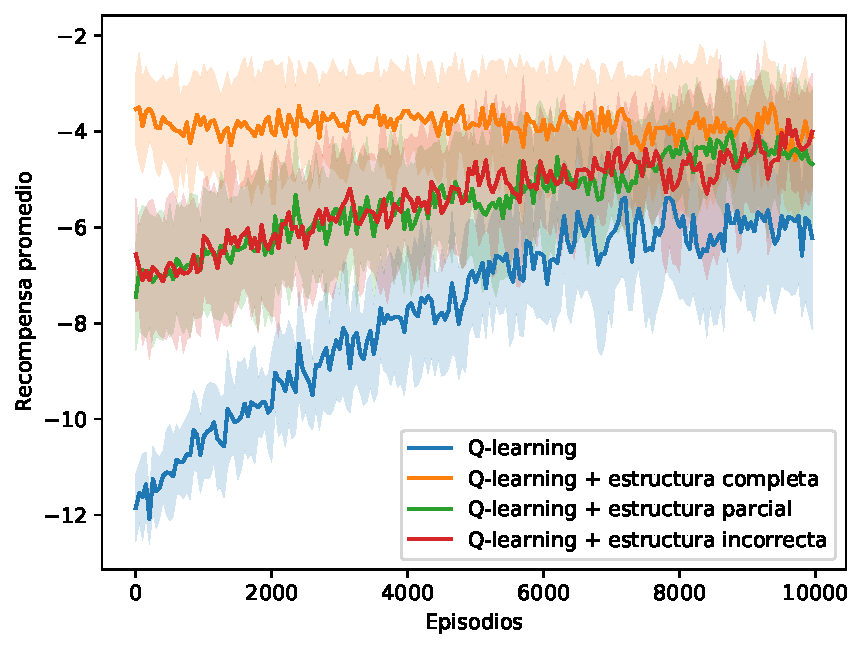
\includegraphics[width=.32\linewidth]{Chapter5/Figs/modexp/stochastic_medium_05_one_to_many_N_7_experiments_10_episodes_10000_eps_35000.pdf}&
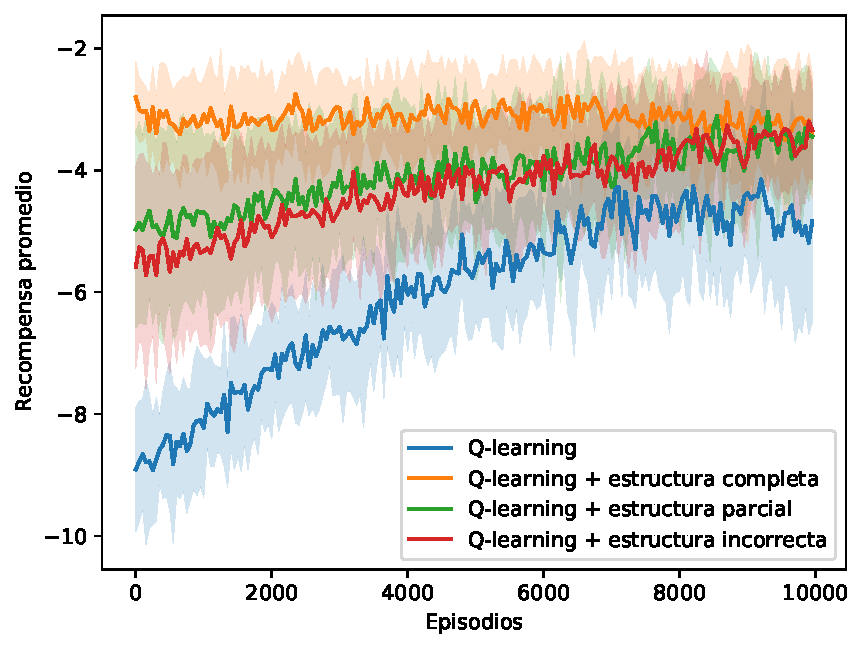
\includegraphics[width=.32\linewidth]{Chapter5/Figs/modexp/stochastic_medium_05_many_to_one_N_7_experiments_10_episodes_10000_eps_35000.pdf}
\\
\rowname{$N = 9$}&

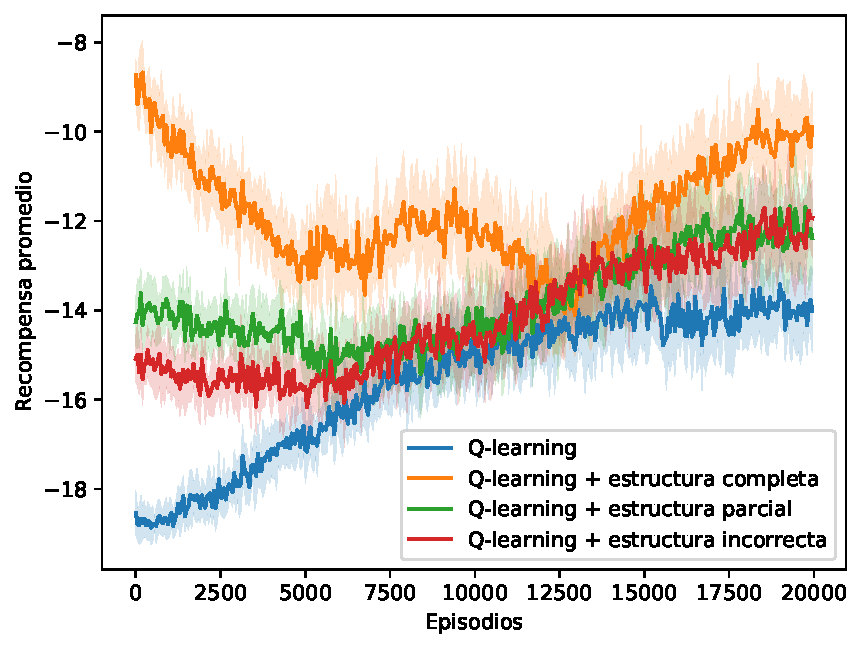
\includegraphics[width=.32\linewidth]{Chapter5/Figs/modexp/stochastic_medium_05_one_to_one_N_9_experiments_10_episodes_20000_eps_90000.pdf}&
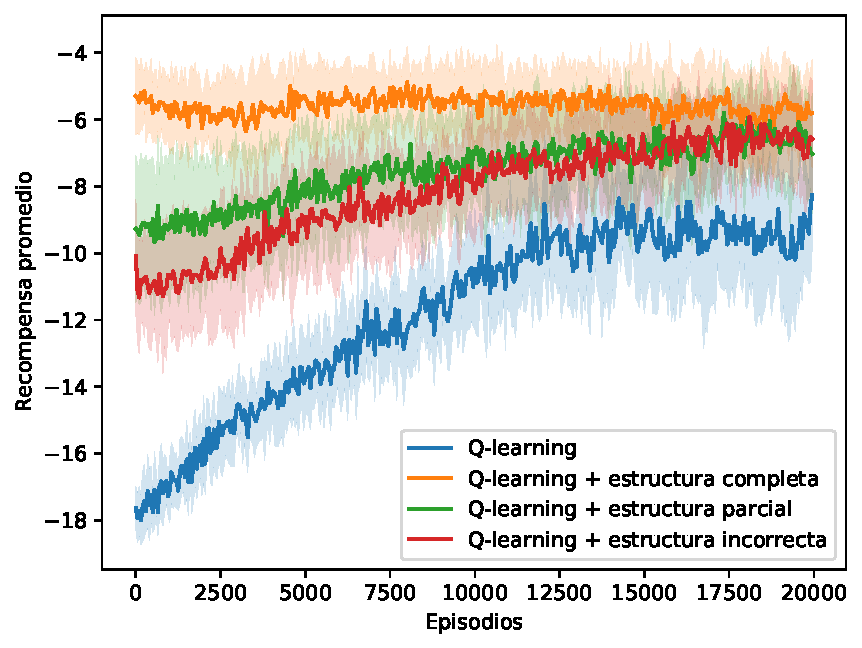
\includegraphics[width=.32\linewidth]{Chapter5/Figs/modexp/stochastic_medium_05_one_to_many_N_9_experiments_10_episodes_20000_eps_90000.pdf}&
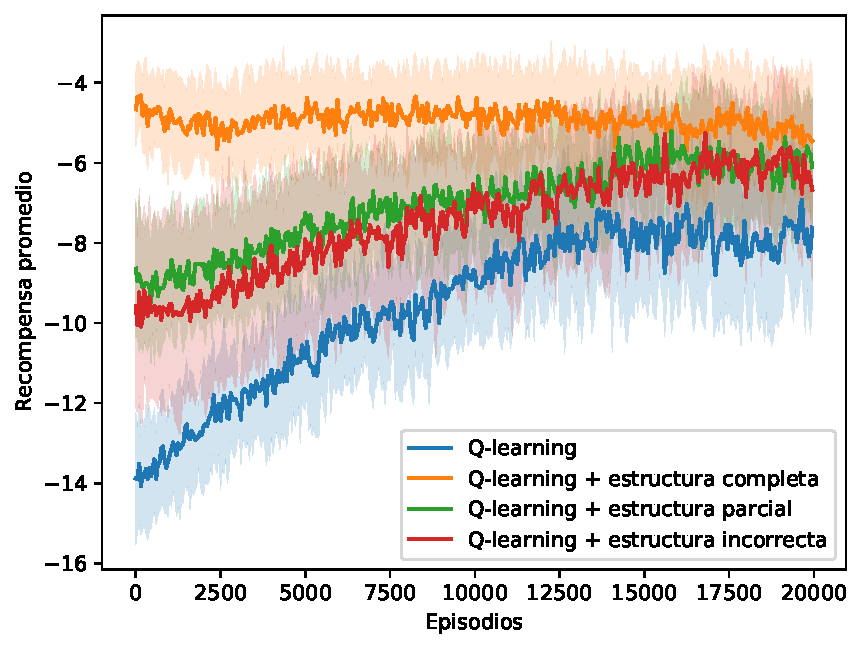
\includegraphics[width=.32\linewidth]{Chapter5/Figs/modexp/stochastic_medium_05_many_to_one_N_9_experiments_10_episodes_20000_eps_90000.pdf}

\end{tabular}
\caption{Comparación del desempeño para los 4 algoritmos con un nivel de alteración $p_{mod} = 50 \%$ en un ambiente estocástico. Las gráficas muestran la medida $average$ y la desviación estándar (región sombreada)para 10 experimentos con 10000 (para $N = 5, 7$) y 20000 (para $N = 9$) episodios.}
\label{fig:med-mod-sto}
\end{figure}



\begin{figure}
\settoheight{\tempdima}{\includegraphics[width=.32\linewidth]{example-image-a}}%
\centering\begin{tabular}{@{}c@{ }c@{ }c@{ }c@{}}
&\textbf{Uno-a-uno} & \textbf{Causa común} & \textbf{Efecto común} \\
\rowname{$N = 5$}&
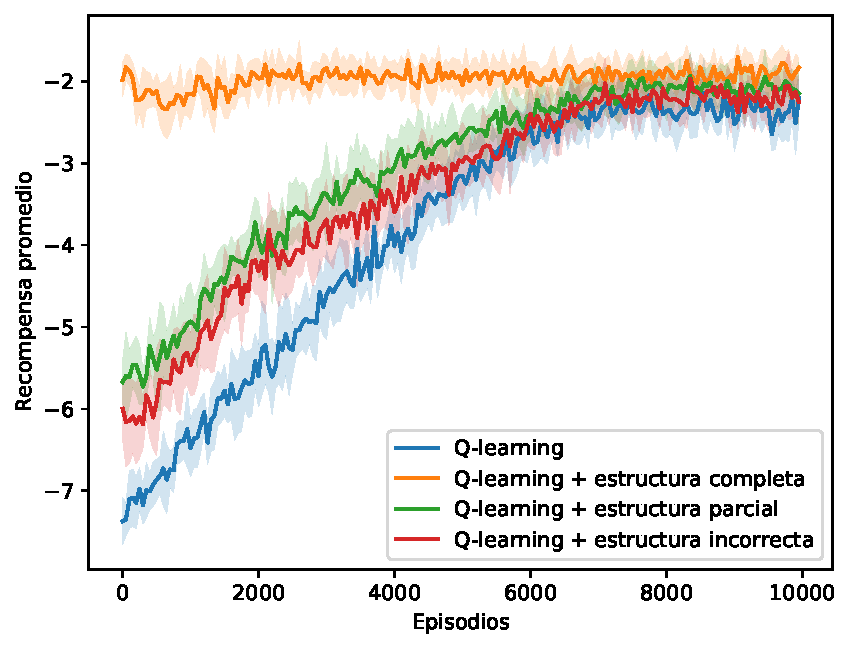
\includegraphics[width=.32\linewidth]{Chapter5/Figs/modexp/deterministic_high_075_one_to_one_N_5_experiments_10_episodes_10000_eps_25000.pdf}&
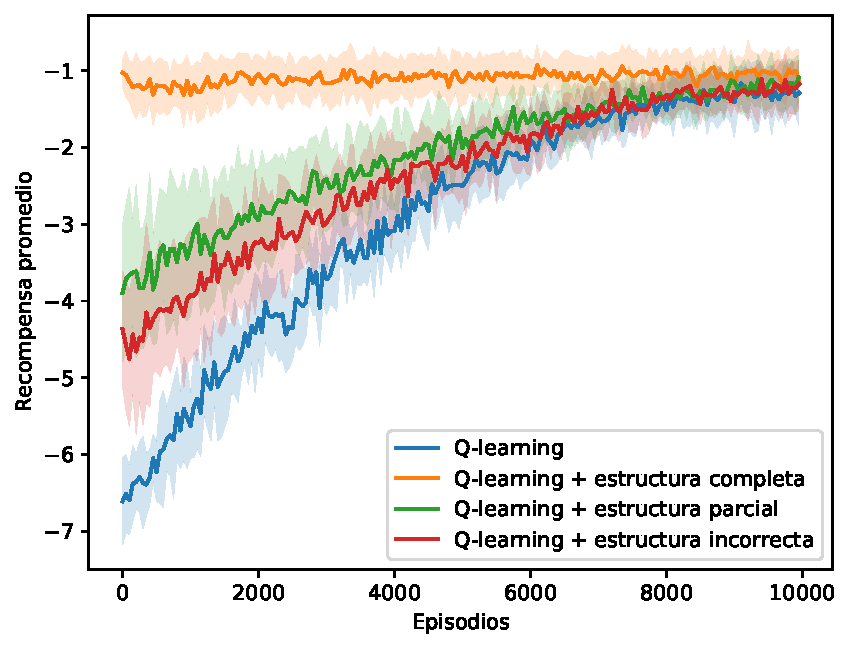
\includegraphics[width=.32\linewidth]{Chapter5/Figs/modexp/deterministic_high_075_one_to_many_N_5_experiments_10_episodes_10000_eps_25000.pdf}&
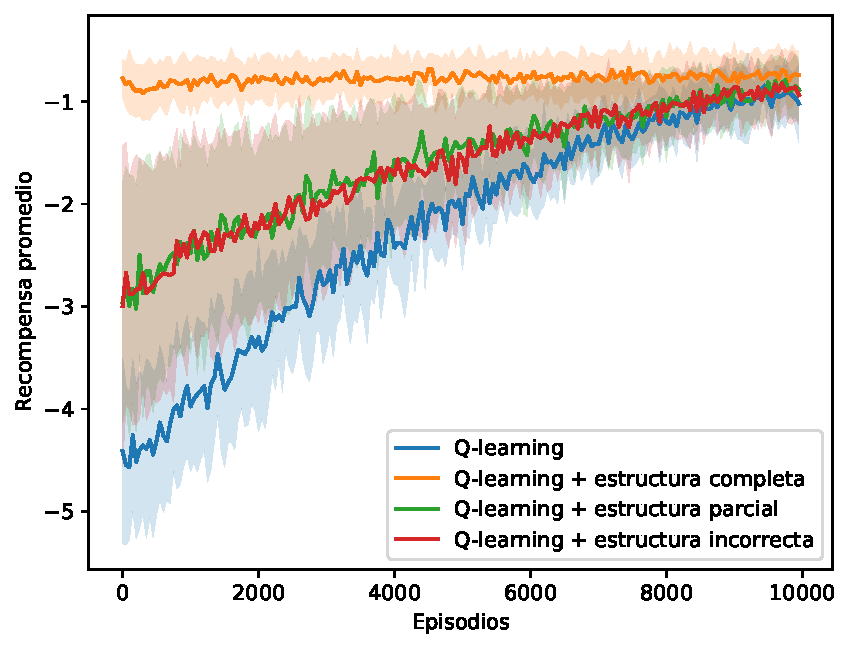
\includegraphics[width=.32\linewidth]{Chapter5/Figs/modexp/deterministic_high_075_many_to_one_N_5_experiments_10_episodes_10000_eps_25000.pdf}
\\
\rowname{$N=7$}&
\includegraphics[width=.32\linewidth]{Chapter5/Figs/modexp/deterministic_high_075_one_to_one_N_7_experiments_10_episodes_10000_eps_35000.pdf}&
\includegraphics[width=.32\linewidth]{Chapter5/Figs/modexp/deterministic_high_075_one_to_many_N_7_experiments_10_episodes_10000_eps_35000.pdf}&
\includegraphics[width=.32\linewidth]{Chapter5/Figs/modexp/deterministic_high_075_many_to_one_N_7_experiments_10_episodes_10000_eps_35000.pdf}
\\
\rowname{$N = 9$}&

\includegraphics[width=.32\linewidth]{Chapter5/Figs/modexp/deterministic_high_075_one_to_one_N_9_experiments_10_episodes_20000_eps_90000.pdf}&
\includegraphics[width=.32\linewidth]{Chapter5/Figs/modexp/deterministic_high_075_one_to_many_N_9_experiments_10_episodes_20000_eps_90000.pdf}&
\includegraphics[width=.32\linewidth]{Chapter5/Figs/modexp/deterministic_high_075_many_to_one_N_9_experiments_10_episodes_20000_eps_90000.pdf}


\end{tabular}

\caption{Comparación del desempeño para los 4 algoritmos con un nivel de alteración $p_{mod} = 75 \%$ en un ambiente determinista. Las gráficas muestran la medida $average$ y la desviación estándar (región sombreada) para 10 experimentos con 10000 (para $N = 5, 7$) y 20000 (para $N = 9$) episodios.}
\label{fig:high-mod-det}
\end{figure}

\begin{figure}
\settoheight{\tempdima}{\includegraphics[width=.32\linewidth]{example-image-a}}%
\centering\begin{tabular}{@{}c@{ }c@{ }c@{ }c@{}}
&\textbf{Uno-a-uno} & \textbf{Causa común} & \textbf{Efecto común} \\
\rowname{$N = 5$}&
\includegraphics[width=.32\linewidth]{Chapter5/Figs/modexp/stochastic_high_075_one_to_one_N_5_experiments_10_episodes_10000_eps_25000.pdf}&
\includegraphics[width=.32\linewidth]{Chapter5/Figs/modexp/stochastic_high_075_one_to_many_N_5_experiments_10_episodes_10000_eps_25000.pdf}&
\includegraphics[width=.32\linewidth]{Chapter5/Figs/modexp/stochastic_high_075_many_to_one_N_5_experiments_10_episodes_10000_eps_25000.pdf}
\\
\rowname{$N=7$}&
\includegraphics[width=.32\linewidth]{Chapter5/Figs/modexp/stochastic_high_075_one_to_one_N_7_experiments_10_episodes_10000_eps_35000.pdf}&
\includegraphics[width=.32\linewidth]{Chapter5/Figs/modexp/stochastic_high_075_one_to_many_N_7_experiments_10_episodes_10000_eps_35000.pdf}&
\includegraphics[width=.32\linewidth]{Chapter5/Figs/modexp/stochastic_high_075_many_to_one_N_7_experiments_10_episodes_10000_eps_35000.pdf}
\\
\rowname{$N = 9$}&

\includegraphics[width=.32\linewidth]{Chapter5/Figs/modexp/stochastic_high_075_one_to_one_N_9_experiments_10_episodes_20000_eps_90000.pdf}&
\includegraphics[width=.32\linewidth]{Chapter5/Figs/modexp/stochastic_high_075_one_to_many_N_9_experiments_10_episodes_20000_eps_90000.pdf}&
\includegraphics[width=.32\linewidth]{Chapter5/Figs/modexp/stochastic_high_075_many_to_one_N_9_experiments_10_episodes_20000_eps_90000.pdf}
\end{tabular}

\caption{Comparación del desempeño para los 4 algoritmos con un nivel de alteración $p_{mod} = 75 \%$ en un ambiente estocástico. Las gráficas muestran la medida $average$ y la desviación estándar (región sombreada) para 10 experimentos con 10000 (para $N = 5, 7$) y 20000 (para $N = 9$) episodios.}
\label{fig:high-mod-sto}
\end{figure}


